\documentclass[
  bibliography=totoc,
  listof=totoc,
  oneside,
]{scrbook}

\usepackage[utf8]{inputenc} % Use UTF-8 as input file encoding
\usepackage[T1]{fontenc} % Use Type 1 (8bit) fonts
\usepackage[ngerman,american]{babel} % Language settings

\usepackage[
  style=numeric-comp,
  backref=true,
]{biblatex}
\addbibresource{stuff.bib}

\usepackage{todonotes}

\usepackage{etoolbox} % \ifblank
\usepackage{xparse} % \NewDocumentCommand
\usepackage{mathtools} % Math improvements, loads amsmath
\usepackage{amssymb} % \mathbb
\usepackage{amsthm}
\usepackage{thmtools} % \listoftheorems
\usepackage{array} % >{...} column modifiers
\usepackage{siunitx}
\usepackage{booktabs} % \toprule etc
\usepackage{xspace}
\usepackage{enumitem} % improved listings: \setlist
\usepackage{listings,xcolor} % source code
\usepackage{subcaption} % subfigure
\usepackage[nottoc]{tocbibind} % remove toc from toc (caused by algorithm2e)
\usepackage[
  linesnumbered,
  algochapter,
  dotocloa,
  norelsize, % line numbers in \scriptsize
]{algorithm2e}

% hyperref should be loaded last
\usepackage[
  bookmarksopen,
  bookmarksopenlevel=0, % close all
  bookmarksnumbered,
]{hyperref}

% glossaries must be loaded after hyperref
\usepackage[toc,shortcuts]{glossaries}

\mathtoolsset{
  %showonlyrefs,
  showmanualtags,
}

\sisetup{
  binary-units,
  round-mode = places,
  round-precision = 2,
}

\hypersetup{
  %hidelinks, %TODO: activate me for print version
}

\usetikzlibrary{graphs,arrows.meta}
\tikzset{>=Stealth}

% hyperref/babel/koma
\renewcaptionname{american}\chapterautorefname{Chapter}
\renewcaptionname{american}\sectionautorefname{Section}
\renewcaptionname{american}\subsectionautorefname{Subsection}
\newcaptionname{american}\algorithmcflinename{step} % algorithm2e

\newcommand{\N}{\mathbb{N}} % Natural numbers
\newcommand{\Z}{\mathbb{Z}} % Whole numbers
\newcommand{\Q}{\mathbb{Q}} % Rational numbers
\newcommand{\R}{\mathbb{R}} % Real numbers
\newcommand{\C}{\mathbb{C}} % Complex numbers
\newcommand{\F}{\mathbb{F}} % Arbitrary Field
\newcommand{\K}{\mathbb{K}} % Arbitrary Field

\newcommand{\Cneg}{\C_-} % Negative Half Plane

\newcommand{\im}{i} % imaginary unit

\newcommand{\onehalf}{\tfrac{1}{2}}

% matrices
\newcommand\Cnn{\C^{n\times n}}
\newcommand\Rnn{\R^{n\times n}}
\newcommand\Rnr{\R^{n\times r}}
\newcommand\Rnk{\R^{n\times k}}
\newcommand\Rkk{\R^{k\times k}}
\newcommand\nnz{\operatorname{nnz}}
\renewcommand\vec{\operatorname{vec}}
\DeclareMathOperator{\colspan}{span}
\DeclareMathOperator{\orth}{orth}
\DeclareMathOperator{\rank}{rank}
\DeclareMathOperator{\diag}{diag}
\newcommand\MP{\dagger} % Moore Penrose pseudo-inverse

% transpose and conjugate/Hermitian transpose:
\newcommand\conj[1]{\overline{\optional{#1}}}
\newcommand\T{T}
\newcommand\HT{H}

% Rosenbrock
\newcommand\Ham{\ensuremath{H}}
\newcommand\Ricc{\operatorname{\mathcal R}}
\newcommand\Jac{\operatorname{\mathcal J}}

 % ADI
\newcommand\Aip{\mathop{H_k^+}}
\newcommand\Aim{\mathop{H_k^-}}
\newcommand\Aipm{\mathop{H_k^\pm}}
\newcommand\Aiip{\mathop{V_k^+}}
\newcommand\Aiim{\mathop{V_k^-}}
\newcommand\Aiipm{\mathop{V_k^\pm}}
\newcommand\Cayley{\mathop{\mathcal{C}}}
\newcommand\Aipinv{\mathop{(\Aip)^{-1}}}
\newcommand\Aiipinv{\mathop{(\Aiip)^{-1}}}
\newcommand\Lyap{\operatorname{\mathcal L}}

% usage: \{2x\given x\in\N}
\newcommand{\given}{\mid}

% usage: \Set[\big]{2x \given x\in\N}
\newcommand\SetSymbol[1][]{%
  \nonscript\:#1\vert
  \allowbreak
  \nonscript\:
  \mathopen{}}
\DeclarePairedDelimiterX{\Set}[1]{\lbrace}{\rbrace}{%
  \renewcommand\given{\SetSymbol[\delimsize]}% this effect is local only
  #1%
}

% personal taste:
\let\epsilon\varepsilon
%\renewcommand{\to}{\longrightarrow}
%\renewcommand{\mapsto}{\longmapsto}
%\renewcommand{\gets}{\longleftarrow}
\renewcommand{\Re}{\operatorname{Re}} % real part of a complex number
\renewcommand{\Im}{\operatorname{Im}} % imaginary part

% some more delimiters:
\NewDocumentCommand{\optional}{m}{\ifblank{#1}{\,\cdot\,}{#1}}
\DeclarePairedDelimiterX{\abs}[1]{\lvert}{\rvert}{\optional{#1}}
\DeclarePairedDelimiterX{\norm}[1]{\lVert}{\rVert}{\optional{#1}}
\DeclarePairedDelimiterX{\scalar}[2]{\langle}{\rangle}{\optional{#1},\optional{#2}}
\newcommand{\card}{\abs}

% integration:
\NewDocumentCommand{\intd}{m}{\,\textup{d}#1}
\newcommand\dt{\intd{t}}

% differentiation:
\NewDocumentCommand{\pdiff}{mm}{\frac{\partial #2}{\partial #1}}
\NewDocumentCommand{\diff}{mm}{\frac{\mathrm{d} #2}{\mathrm{d} #1}}

% https://tex.stackexchange.com/questions/22561/what-is-the-proper-use-of-i-e-backslash-at?noredirect=1&lq=1
\makeatletter % no idea why this is needed. \@ifnextchar doesn't work without it.
\newcommand\cf{cf.\@\xspace} % confer
\newcommand\eg{e.g.\@\xspace} % exempli gratia
\newcommand\etc{etc\@ifnextchar.{}{.\@\xspace}} % et cetera
\newcommand\ie{i.e.\@\xspace} % id est
\newcommand\wrt{w.r.t.\@\xspace} % with respect to
\makeatother

% Remember: use \label{thm:...} for theorems, propositions, lemmata, etc.
% This way the type of an environment can easily be changed.

\declaretheoremstyle[
  spaceabove = \topsep,
  spacebelow = \topsep,
  postheadspace = 0.5em, % matches proof
  headfont = \usekomafont{captionlabel},
  notefont = \normalfont\sffamily,
  bodyfont = \normalfont,
  qed = \ensuremath{\triangle\hspace*{-.1ex}}, % bring it a little bit closer to the edge
]{myplain}

\declaretheoremstyle[
  spaceabove = \topsep,
  spacebelow = \topsep,
  postheadspace = 0.5em, % matches proof
  headfont = \itshape,
  numbered = no,
  qed = \ensuremath{\triangle\hspace*{-.1ex}}, % bring it a little bit closer to the edge
]{myremark}

\renewcommand{\qedsymbol}{\ensuremath{\square}} %TODO: still not bold enough compared to \triangle

\declaretheorem[style=myplain, numberwithin=chapter]{lemma}
\declaretheorem[style=myplain, numberlike=lemma]{corollary}
\declaretheorem[style=myplain, numberlike=lemma]{proposition}
\declaretheorem[style=myplain, numberlike=lemma]{theorem}
\declaretheorem[style=myplain, numberlike=lemma]{hypothesis}

\declaretheorem[style=myplain, numberlike=lemma]{definition}
\declaretheorem[style=myplain, numberlike=lemma]{example}

\declaretheorem[style=myremark]{remark}


% ******************************************************************************
% Listings

\setlist[enumerate]{font=\normalfont}
\setlist[enumerate,1]{label=(\roman*)}
\setlist[enumerate,2]{label=(\alph*)}
\setlist[enumerate,3]{label=(\arabic*)}


% ******************************************************************************
% Source Code

\renewcommand{\lstlistlistingname}{List of Code Snippets}
\renewcommand{\lstlistingname}{Code Snippet}

\lstset{
  basicstyle=\small\ttfamily,
  numberstyle=\scriptsize\sffamily, % matches algorithm2e
  numbers=left,
  % use special julia comments as range markers: #== text ==#
  rangeprefix=\#\=\=\ ,
  rangesuffix=\ \=\=\#,
  includerangemarker=false,
  % add latex labels using #* \label{line:...}
  escapeinside={\#*}{\^^M},
}

% ******************************************************************************
% algorithm2e

\setlength{\algomargin}{0pt}

\newcommand{\komacaptionsty}{\usekomafont{captionlabel}}
\SetAlCapFnt{\usekomafont{captionlabel}}
\SetNlSty{textsf}{}{} % matches listings
\SetKwSty{komacaptionsty}
\SetCommentSty{normalfont}
\SetArgSty{normalfont} % used for conditions as well

\makeatletter
% Fix alignment of listofalgorithms:
\renewcommand*\l@algocf{\@dottedtocline{1}{1.5em}{2.3em}}
% Thanks to https://tex.stackexchange.com/a/147750/95100
\renewcommand{\@algocf@capt@plain}{above}% formerly {bottom}
\makeatother

\AtBeginDocument{
  \DontPrintSemicolon
  \SetAlgorithmName{Algorithm}{Algorithm}{List of Algorithms}
  \SetKwComment{Comment}{}{}
}

\newcommand\julia\texttt
\newcommand\code\texttt

\newcommand\LDLt{LDL\textsuperscript{T}}

\counterwithout*{footnote}{chapter}
\setcounter{topnumber}{1} % max number of floats at top of page
\renewcommand{\bottomfraction}{0.5}
\renewcommand{\listtheoremname}{List of Theorems and Examples}

\newcommand\LandauO{\operatorname{\mathcal O}}

% runtime estimates
\newcommand\hattpar{\hat t_\text{par}} % estimate
\newcommand\hattseq{\hat t_\text{seq}} % estimate
\newcommand\tpar{t_\text{par}}
\newcommand\tseq{t_\text{seq}}
\newcommand\twarmup{t_\text{warm-up}}
\newcommand\trampup{t_\text{ramp-up}}
\newcommand\JIT{\operatorname{compile}}

% error estimates
\newcommand\umach{\mathrm u_\text{mach}} % machine precision


\makeglossaries

\begin{document}

% -----------------------------------------------------------------------------
\frontmatter

\chapter{Abstract}

Get a parareal solver running with column compression.
The tricky part is that the interface solutions (solutions at time slice bounds) differ in size,
\wrt both storage requirements and matrix dimensions.


\cleardoublepage
\pdfbookmark{\contentsname}{toc}
\tableofcontents
\listoffigures

\cleardoublepage
\pdfbookmark{\listtheoremname}{loe}
\listoftheorems

\listoftodos
\todototoc

% -----------------------------------------------------------------------------
\mainmatter
\chapter{Introduction}

The implementations of the parareal scheme and \ac{DRE} solver must be composable and,
therefore, independent from one another.

The \ac{DRE} arises in \eg optimal control of \ac{LTI} systems, \cf \autoref{sec:basics:HJT},
optimal filtering, $H_\infty$ control of \ac{LTV} systems.

\section*{Hardware and Software Used}

Up to 29 nodes (450 cores) of the linux cluster Mechthild\footnote{\url{https://www.mpi-magdeburg.mpg.de/cluster/mechthild}}
at the Max Planck Institute for Dynamics of Complex Technical Systems in Magdeburg, each having ...

Unless stated otherwise, each process uses a single thread.

my private laptop (MacBook Pro 13-inch, 2018, macOS 11)

\julia{Makie.jl} \cite{Makie} to create most images

\julia{DrWatson.jl} \cite{DrWatson} to assist data management.

\julia{DifferentialEquations.jl} \cite{DifferentialEquations} for \autoref{example:parareal}

\section*{Acknolegdements?}

I would like to thank ...


\chapter{Mathematical Basics}
\section{Linear Systems and Related Matrix Equations}
\section{Hamilton-Jacobi Theory}

\chapter{Large-Scale Matrix Equations}

\section{Sparse Matrices}
Describe data structures to store sparse matrices.

\begin{example}[Non-zeros of Steel Profile]
  The Steel Profile of the Oberwolfach Benchmark Collection of size $n=371$
  contains of sparse matrices having
  $\nnz(E) = 2343$ or \SI{1.7}{\percent},
  $\nnz(A) = 2341$ or \SI{1.7}{\percent}, and
  $\nnz(B) = 87$ or \SI{3.4}{\percent} non-zero entries.
  Although not being stored sparsely, $\nnz(C) = 17$ or \SI{0.8}{\percent}.
\end{example}

Even if the system matrices $E, A, B, C$ are sparse,
the solution $X$ is dense.
However, it usually is of low numerical rank.

\section{Low-Rank Representations}

\todo{Find reference. Max Behr had a slide on that in his defense.}
\begin{theorem}[Low-Rank Solutions]
\label{thm:lowrank}
The solution $X$ to a \ac{DRE} is of low numerical rank.
\end{theorem}

Briefly describe classical Cholesky-type factorization, $X=ZZ^\T$.
This does only exist for symmetric positive-definite matrices $X$.

\todo[inline]{Decide on how to call the low-rank factors: $ZZ^\T$ vs $QQ^\T$.}
\todo[inline]{Decide on how to call the low-rank factors: $LDL^\T$ vs $QSQ^\T$.}

$Z$ and $L \in \R^{n\times r}$ are not necessarily triangular,
though there exist equivalent triangular decompositions.

\begin{proposition}[Triangular Low-Rank Factorizations]
  Let $X=ZZ^\T$ or $X=ZDZ^\T$ for some $Z\in\R^{n\times r}$ and $D\in\R^{r\times r}$,
  $r \leq n$,
  then there exist a lower triangular $\hat{Z}$
  and some $\hat D$ of the same size satisfying
  $X=\hat Z \hat Z^\T$
  or $X=\hat Z \hat D \hat Z^\T$.
\end{proposition}
\begin{proof}
  We are looking for a transformation $H\in\R^{r\times r}$ such that $\hat Z := ZH$ is triangular and $HH^\T = I_r$.
  Then $\hat Z := ZH$ and $\hat D := H^\T DH$ have the desired properties.

  \todo{How to handle row permutations?}
  Without loss of generality, let the first $r$ rows of $Z$ have full rank.
  Let $z_1\in\R^r$ denote the first row of $Z$.
  Let $H_r\in\R^{r\times r}$ be the \Householder transformation mapping
  $z_1$ onto $\norm{z_1}e_1 = (\norm{z_1},0,\ldots) \in \R^r$, \ie
  \begin{equation}
    H_r := I_r - \frac{2}{v^\T v} vv^T
  \end{equation}
  for $v := z_1 - \norm{z_1}e_1$.
  Note that $H_r H_r^\T = I_r$ and $H_r = H_r^\T$.
  As $Z$ has full rank, $v \neq 0$ and $H_r$ is well defined.
  Indeed,
  \begin{equation*}
    H_r z_1
    = z_1 - \frac{2v^\T z_1}{v^\T v} \cdot v
    = z_1 - 1 \cdot v
    = \norm{z_1}e_1
  \end{equation*}
  such that
  \begin{equation}
    Z H_r = (H_r Z^\T) = \begin{pmatrix}
      \norm{z_1} & 0 \\
      Z_{12} & Z_{22}
    \end{pmatrix}
  \end{equation}
  for some $Z_{12} \in \R^{n-1 \times 1}$ and $Z_{22} \in \R^{n-1 \times r-1}$.

  Similarly, let $z_2\in\R^{r-1}$ denote the first row of $Z_{22}$ and
  let $H_{r-1} \in \R^{r-1 \times r-1}$ be the \Householder matrix mapping
  $z_2$ onto $\norm{z_2}e_1 \in\R^{r-1}$.
  This iteratively defines the matrix
  \begin{equation}
    H :=
    H_r \cdot
    \begin{pmatrix}
      I_1 \\ & H_{r-1}
    \end{pmatrix}
    \cdots
    \begin{pmatrix}
      I_{r-2} \\ & H_2
    \end{pmatrix}
    .
  \end{equation}

  Note that $H_1 = I_1$ or $H_1 = -I_1$,
  which therefore isn't needed for the transformation into a triangular matrix.
  Further, note that every factor in the product above is itself a \Householder transformation acting on $\R^r$,
  whose corresponding vector has its leading components filled with zeros.
\end{proof}

\todo[inline]{%
  The theorem above doesn't help / is misleading.
  It's better to defer the reader to the compression section.
}

\subsection{Low-Rank Update Formula}
\label{sec:lr:update}

Let $A, B \in\R^{n\times r}$ and $C, D\in\R^{r\times r}$.
While an update for the \ac{LRCF} is straight-forward,
\begin{equation}
  AA^\T + BB^\T =
  \begin{bmatrix}
    A & B
  \end{bmatrix}
  \begin{bmatrix}
    A^\T \\ B^\T
  \end{bmatrix}
  ,
\end{equation}
a downdate is more involved.
One option is to use complex arithmetic, \ie
\begin{equation}
  AA^\T - BB^\T =
  \begin{bmatrix}
    A & \im B
  \end{bmatrix}
  \begin{bmatrix}
    A^\T \\ \im B^\T
  \end{bmatrix}
\end{equation}
where $\im^2=-1$.
This has several drawbacks.
The mathematical one is that we expect a real-valued\todo{Do we?}\ solution to the \ac{DRE}.
Hence, the imaginary part should converge to zero quickly,
or there should be an equivalent real-valued factorization.
This leads to two technical drawbacks.
Firstly, the complex arithmetic should not be necessary everywhere,
switching back to real arithmetic is highly non-trivial.\footnote{Don't be clever / KISS!}
\todo{Find reference!}
Secondly, complex arithmetic is inefficient, \ie has a more than the to-be-expected 2x penalty compared to real arithmetic.

Another option is to handle the parts separately which are added versus subtracted in the superposition,
and compute the difference afterwards.
While this may only require updates,
the overall result suffers from numerical cancellation
\cite[50]{Lang2015}
\cite[\pno~186, thesis~10]{Lang2017}.

A different strategy to represent matrices of low numerical rank is the \ac{LRSIF} \cite{Benner2009,Lang2015},
which does not require up- and downdate to be handled separately:
\begin{equation}
  ACA^\T \pm BDB^\T =
  \begin{bmatrix}
    A & B
  \end{bmatrix}
  \begin{bmatrix}
    C \\ & \pm D
  \end{bmatrix}
  \begin{bmatrix}
    A^\T \\ B^\T
  \end{bmatrix}
\end{equation}
The resulting low-rank object $QSQ^\T$ consists of much larger matrices,
$Q \in\R^{n\times 2r}$ and $S\in\R^{2r\times 2r}$.
Having \autoref{thm:lowrank} in mind,
and with iterative algorithms in sight,
the inner dimension must not grow arbitrarily.

\subsection{Column Compression}
\label{sec:lr:compression}

maximum-rank truncation,
singular value tolerance,
...

\todo{use proper algorithm}
Taken from \cite[Section 6.3.3]{Lang2017}:
Given $GSG^\T$, $G\in\Rnk$, and a tolerance $\epsilon\in\R$,
compute $G_rS_rG_r^\T \approx GSG^\T$, $G_r\in\Rnr$.
\begin{enumerate}
  \item
    Compute $G=QR\Pi^\T$ with $Q\in\Rnk$, $R\in\Rkk$ and a permutation $\Pi\in\Rkk$.
  \item
    Compute a decomposition $R \Pi^\T S \Pi R^\T = V \Lambda V^\T$ with $V \in \Rkk$
    and a diagonal matrix $\Lambda\in\Rkk$ with diagonal entries $\abs{\lambda_1}\geq\ldots\geq\abs{\lambda_k}$.
  \item
    Set $G_r := QV_r \in\Rnr$ and $S := \Lambda_r$ with $r\leq k$ and $\abs{\lambda_{r+1}}\leq\epsilon$.
    $V_r$ consists of the first $r$ columns of $V$ and $\Lambda_r$ of the first diagonal block of $\Lambda$.
\end{enumerate}

\todo[inline]{%
The algorithm above uses an absolute cut-off $\epsilon$.
How to integrate $G,S$ into a relative cut-off?
Maybe a \enquote{cheap} adaptation of \cite[Algorithm~2.2, line~2]{Lang2017},
or the even simpler $\epsilon\abs{\lambda_1}$?
}

\section{Model Order Reduction}
Give brief overview.
Details out of scope.
Assume problem to be given in reduced form;
solving the reduced order model then requires same algorithms/techniques.

\chapter{Parareal Method}
\label{sec:pr}

The parareal method is a parallel-in-time integration scheme to solve \acp{ODE}.
It goes back to \citeauthor{Lions2001}~\cite{Lions2001},
though the most common form also used in this thesis first appeared in \citeauthor{Baffico2002}~\cite{Baffico2002}.
In this chapter we'll first describe the general properties of the parareal method,
and derive it as a Newton method following \cite{Gander2007}.
Lastly, in \autoref{sec:pr:DRE} we'll adapt the method for \acp{LRSIF}.

\section{Overview}
\label{sec:pr:properties}

Consider the autonomous \ac{IVP}
\begin{equation}
  \label{eq:IVP}
  \left\{
  \begin{aligned}
    \dot u &= f(u) \\
    u(t_0) &= u_0
  \end{aligned}
  \right.
\end{equation}
over the time span $[t_0, t_f]$.
In practical applications,
one is typically interested in a high temporal resolution trajectory of $u$.
Let $F(t, t_0, u_0) \approx u(t)$ be such a fine/high-precision solver for the \ac{IVP} above.
However, applying $F$ to the whole time span may be too slow.
The goal therefore is to apply $F$ on several time slices $[t_{n-1}, t_n]$ in parallel,
$1 \leq n \leq N$,
with the help of a faster but lower-precision solver $G(t, t_0, u_0) \approx u(t)$.
Therefore, fix a coarse discretization $t_0 < t_1 < \ldots < t_N = t_f$.
Then the parareal method to compute $U_n \approx u(t_n)$ reads
\begin{equation}
  \label{eq:pr:method}
  \left\{
  \begin{aligned}
    U^0_{n+1} &:= G(U^0_n) \\
    U^{k+1}_{n+1} &:= G(U^{k+1}_n) + F(U^k_n) - G(U^k_n)
  \end{aligned}
  \right.
\end{equation}
where $U^0_0 := u_0$ and $G(U_n) := G(t_{n+1}, t_n, U_n)$,
$F(U_n) := F(t_{n+1}, t_n, U_n)$
integrate from~$t_n$ to~$t_{n+1}$.
The general data dependencies between the parareal iterates~$U_n^k$
are shown in \autoref{fig:pr:DAG}.
Observe that in any topological order of that graph,
the coarse solutions $G(U_n^k)$ for any fixed~$k$ need to be computed sequentially over $n$.

Notice how in general each coarse solution $G(\optional{})$ is needed twice.
Therefore, a reasonable scheduling pattern of the directed acyclic graph of \autoref{fig:pr:DAG}
that exploits good data locality is a pipeline of stages $n$ which compute
\begin{equation}
\label{eq:pr:stage}
  \begin{tikzpicture}[
    baseline=(Un1k1.base),
    text height=1.5ex,
    text depth=0.25ex,
  ]
    \graph[grow right sep=0] {
      ""/"\ldots,"
      -!- Gnk1/"$G(U_{n-1}^{k})$\rlap{,}"
      -!- Un1k1/"$U_{n}^{k}$\rlap{,}"
      -!- Fnk/"$F(U_{n-1}^{k})$,"
      -!- ""/"\ldots,"
    };
    \draw[<-] (Gnk1) -- +(70:-1cm);
    \draw[->] (Un1k1) -- +(70:1cm);
  \end{tikzpicture}
\end{equation}
where the arrows denote data dependencies or transmissions from and to the adjacent stages.
Dependencies within a stage are not shown.
Note how this pattern correspond to the rows of \autoref{fig:pr:DAG}.
Each stage~$n$ holds~$G(U_{n-1}^{k-1})$ and~$F(U_{n-1}^{k-1})$ in memory,
receives~$U_{n-1}^k$ from its predecessor,
and sends~$U_n^k$ to its successor.
However, there is no need that all stages $n$ compute the same number of refinements $k$,
due to the following proposition.

\begin{figure}[t]
  \centering
  \begin{tikzpicture}[
  text height=1.5ex,
  text depth=0.25ex,
]
  \graph[
    math nodes,
    grow right=2cm,
    diag/.style={bend left, shorten >=2pt},
  ]{
    Unk/"U_{n-1}^{k-1}" [label=above:$\vdots$]
    -> Gnk/"G(U_{n-1}^{k-1})" -> Un1k/"U_{n}^{k-1}" [label=above:$\vdots$]
    -> Gn1k/"G(U_{n}^{k-1})" -> Un2k/"U_{n+1}^{k-1}" [label=above:$\vdots$],
    "" -!- Fnk/"F(U_{n-1}^{k-1})" -!- "" -!- Fn1k/"F(U_{n}^{k-1})",
    Unk1/"U_{n-1}^{k}"
    -> Gnk1/"G(U_{n-1}^{k})" -> Un1k1/"U_{n}^{k}"
    -> Gn1k1/"G(U_{n}^{k})" -> Un2k1/"U_{n+1}^{k}",
    "" -!- Fnk1/"F(U_{n-1}^{k})" -!- "" -!- Fn1k1/"F(U_{n}^{k})",
    Unk2/"U_{n-1}^{k+1}" [label=below:$\vdots$]
    -> Gnk2/"G(U_{n-1}^{k+1})" -> Un1k2/"U_{n}^{k+1}" [label=below:$\vdots$]
    -> Gn1k2/"G(U_{n}^{k+1})" -> Un2k2/"U_{n+1}^{k+1}" [label=below:$\vdots$];

    Unk -> Fnk -> Un1k1 -> Fn1k1 -> Un2k2;
    Un1k -> Fn1k -> Un2k1;
    Unk1 -> Fnk1 -> Un1k2;
    Gnk -> [diag] Un1k1;
    Gnk1 -> [diag] Un1k2;
    Gn1k -> [diag] Un2k1;
    Gn1k1 -> [diag] Un2k2;
  };
  \node [left=5mm of Unk.center] {$\cdots$};
  \node [left=5mm of Unk1.center] {$\cdots$};
  \node [left=5mm of Unk2.center] {$\cdots$};
  \node [right=5mm of Un2k.center] {$\cdots$};
  \node [right=5mm of Un2k1.center] {$\cdots$};
  \node [right=5mm of Un2k2.center] {$\cdots$};
\end{tikzpicture}

  \caption{Dependencies between parareal values $U^{k}_{n}$}
  \label{fig:pr:DAG}
\end{figure}

\begin{proposition}[Diagonal Convergence]
\label{thm:pr:conv}
  Stage $n$ of the parareal method converges after at most $n$ iterations:
  \begin{equation*}
    U^k_n = U^n_n = F(U^{n-1}_{n-1})
    \quad
    \forall k \geq n
  \end{equation*}
\end{proposition}
\begin{proof}
  Due to $U^k_0 = u_0$ for all $k$,
  it follows by induction $\forall k \geq n$:
  \begin{equation*}
    \begin{array}{r@{}l@{}l@{}l}
      U^{k+1}_{n+1}
      :={} & F(U^k_n) &{}+ G(U^{k+1}_n) &{}- G(U^k_n) \\
      ={}  & F(U^n_n) &{}+ G(U^n_n)     &{}- G(U^n_n)
      = F(U^n_n)
    \end{array}
  \end{equation*}
\end{proof}

The early iterates $U_n^k$ for $k=n$ thus have fewer dependencies between them,
\cf \autoref{fig:pr:DAG:early}.
Furthermore, the same reasoning as in the proof of \autoref{thm:pr:conv} can
be applied if stage $n$ converges after refinement $k < n$,
\ie $U^{k+1}_n \approx U^k_n$.
In that case, stage $n+1$ converges the refinement thereafter,
\begin{equation}
  \begin{array}{r@{}l@{}l@{}l}
    U^{k+1}_{n+1}
    :={}      & F(U^k_n) &{}+ G(U^{k+1}_n) &{}- G(U^k_n) \\
    \approx{} & F(U^k_n) &{}+ G(U^k_n)     &{}- G(U^k_n)
    = F(U^k_n)
    .
  \end{array}
\end{equation}
Therefore,
assuming $G$ is well conditioned,
there is no need to compute $G(U^{k+1}_n)$.

\begin{figure}[t]
  \centering
  \begin{tikzpicture}[
  text height=1.5ex,
  text depth=0.25ex,
]
  \graph[
    math nodes,
    grow right=2cm,
    diag/.style={bend left, shorten >=2pt},
    ghost/.style={gray},
    eq/.style={double, double distance=2pt, shorten >=0.5ex, shorten <=0.5ex},
  ]{
    Unk/"U_0^0"
    -> Gnk/"G(U_0^0)" -> Un1k/"U_1^0"
    -> Gn1k/"G(U_1^0)" -> Un2k/"U_2^0",
    Unk1/"U_0^1" [ghost, label={[gray]below:$\vdots$}]
    -!- Fnk/"F(U_0^0)" -!- "" -!- Fn1k/"F(U_1^0)",
    "" -!- "" -!- Un1k1/"U_1^1"
    -> Gn1k1/"G(U_1^1)" -> Un2k1/"U_2^1",
    "" -!- "" -!- Un1k2/"U_1^2" [ghost, label={[gray]below:$\vdots$}]
    -!- Fn1k1/"F(U_1^1)",
    "" -!- "" -!- "" -!- "" -!- Un2k2/"U_2^2";

    Unk -> Fnk -> Un1k1 -> Fn1k1 -> Un2k2;
    Un1k -> Fn1k -> Un2k1;
    Gn1k -> [diag] Un2k1;

    Unk -- [ghost,eq] Unk1;
    Un1k1 -- [ghost,eq] Un1k2;
  };
  \node [right=5mm of Un2k.center] {$\cdots$};
  \node [right=5mm of Un2k1.center] {$\cdots$};
  \node [right=5mm of Un2k2.center] {$\cdots$};
\end{tikzpicture}

  \caption{Dependencies between parareal values $U^0_0, \ldots, U_2^2$}
  \label{fig:pr:DAG:early}
\end{figure}

Following \autoref{thm:pr:conv},
the parareal method converges after $k=N$ iterations at the latest,
at which point the parareal solutions equal the fine solution,
$U_n^N = F(U_{n-1}^N)$ for $1\leq n \leq N$.
In practice, however, it may converge much earlier than that,
\ie~$k\ll N$.
Limiting the number of refinements to~$k\leq K$,
and assuming that $F$, $G$, and communication all take constant time,
the expected timeline of a parareal execution is shown in \autoref{fig:timeline:generic}.
Note how the diagram corresponds to \autoref{fig:pr:DAG};
the slope of the $k=0$ face depends on the runtime of $G$.

\begin{figure}[b]
  \centering
  \begin{tikzpicture}
  %\def\mxscale{0.6}
  \def\myscale{0.6}
%\begin{scope}[xscale=\mxscale]
  % axis and labels
  \node[below] at (5,-0.5*\myscale-0.3) {\footnotesize Wallclock Time};
  \node[rotate=90, above] at (-0.5-0.3,5*\myscale) {\footnotesize Parareal Stage};
\begin{scope}[yscale=\myscale]
  \draw[semithick] (-0.5,-0.5) rectangle (10.5,10.5);
  % timeline diagram
  \draw[thick] (0,0)
    -- node[right] {$k=0$} (2,10)
    -- node[below] {$n=N$} (7.9,10)
    -- (6.3,2)
    -- node[below] {$n=k$} cycle;
  \node[right] at (6.9,5) {$k=K$};
  %\draw[gray,thick,dashed] (6.3,2) -- (9.45,3);
  %\draw[gray,thick,dashed] (7.9,10) -- (9.45,10);
\end{scope}
%\end{scope}
\end{tikzpicture}

  \caption[Schematic parareal timeline]{%
    Schematic parareal timeline.
    Time passed and refinement $k$ both increase to the right,
    the parareal stage $n$ increases to the top.
    The $k=K$ boundary won't be visible if $K\geq N$.
  }
  \label{fig:timeline:generic}
\end{figure}

\begin{example}[Linear \acs*{ODE}]
\label{example:parareal}
  Let $\phi := \frac{1+\sqrt{5}}{2}$ denote the golden ratio and
  let $\kappa := \frac{2}{\pi} \log \phi$.
  Consider the \ac{IVP}
  \begin{equation}
    \label{eq:pr:linear}
    \left\{
    \begin{aligned}
      \dot u &= \begin{bmatrix}
        \kappa & -1 \\
        1 & \kappa
      \end{bmatrix} u \\
      u(0) &= \begin{bmatrix}
        -1 \\ -\kappa
      \end{bmatrix}
    \end{aligned}
    \right.
  \end{equation}
  for $t\in[0,2\pi]$.
  Let $N := 5$, $\tau := 2\pi/N$, and $t_n := n\tau$ for $n\in\Set{0,\ldots,N}$.
  Further, let $F$ and $G$ be implicit Euler schemes using step sizes $\tau/100$ and $\tau$, respectively.
  If the fine solver internally uses a finer mesh,
  by \autoref{thm:pr:conv},
  the global solution $x$ may be retrieved at that fine resolution $\tau/100$.

  \begin{figure}[tb]
    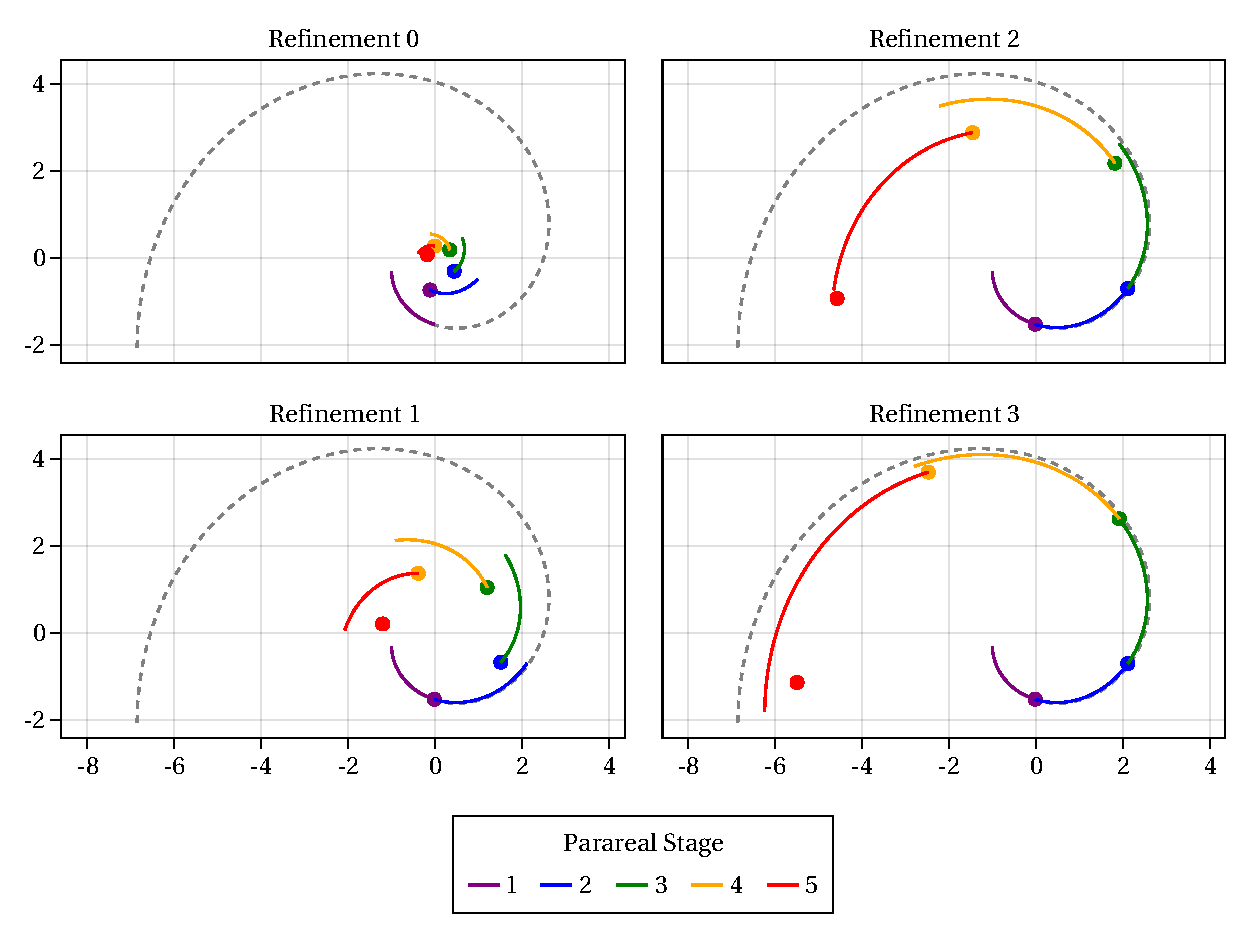
\includegraphics[width=\textwidth]{figures/fig_parareal_example.pdf}
    \caption[Parareal method applied to a linear ODE]{%
      First couple of refinements $k$ of the
      parareal method applied to the linear problem \eqref{eq:pr:linear}.
      The stages $n$ are decoded by color,
      dots denoting $U^k_n$ and lines $F(\optional{}, t_{n-1}, U^k_{n-1})$.
      The dashed gray curve represents the exact solution.
    }
    \label{fig:pr:linear}
  \end{figure}

  \autoref{fig:pr:linear} shows the first couple of iterations of the parareal method applied the problem above.
  For a fixed refinement $k$,
  the values $U^k_n \approx u(t_n)$ (represented by dots) are computed in sequence,
  \cf the horizontal traces in \autoref{fig:pr:DAG}.
  After that, the fine solutions $F(U_n^k)$ (represented by lines) can then be computed in parallel.
  The parareal method only ensures convergence of $U_n^k$.
  Therefore, before convergence is reached,
  the high-resolution trajectories are discontinues at $t_n$.
  Furthermore, note that the overall accuracy of the parareal solution is limited by the accuracy of $F$,
  which explains the remaining gap between the colored and the gray line.
\end{example}

\section{Parareal as a Multiple Shooting Method}
\label{sec:pr:newton}

The following construction is based on \citeauthor{Gander2007}~\cite{Gander2007}.
Consider again the autonomous \ac{IVP}
\begin{equation}
  \tag{\ref*{eq:IVP}}
  \left\{
  \begin{aligned}
    \dot u &= f(u) \\
    u(t_0) &= u_0
  \end{aligned}
  \right.
\end{equation}
Note that the solution $u : [t_0,t_f] \to V $ depends on the initial value $U_0$.
For a discretization $t_0 < t_1 < \ldots < t_N = t_f$
define the local problems
\begin{equation}
  \left\{
  \begin{aligned}
    \dot u_n &= f(u_n) \\
    u_n(t_n) &= U_n
  \end{aligned}
  \right.
\end{equation}
for $n \in \Set{0,\ldots,N-1}$
and determine suitable initial values $U_n$.
Watch the slight abuse of notation in $u_0$
for the initial value $u_0 \in V$
and the solution $u_0 : [t_0,t_1] \to V$ to the first local problem.
The local solutions $u_n : [t_n,t_{n+1}] \to V$ represent a global solution to the \ac{IVP}~\eqref{eq:IVP} if
\begin{equation}
  F(U_0, \ldots, U_{N-1}) :=
  \left(
  \begin{aligned}
    U_0 &- u_0 \\
    U_1 &- u_0(t_1, U_0) \\
    &\vdotswithin{-} \\
    U_{N-1} &- u_{N-2}(t_{N-1}, U_{N-2})
  \end{aligned}
  \right)
  \overset{!}{=} 0.
\end{equation}
Let $U := (U_0, \ldots, U_{N-1})$ and $\mathcal J_F(U)$ denote the Jacobian of $F$ at $U$.
Then, Newton's method reads
\begin{equation}
  U^{k+1} = U^k - \mathop{\mathcal J_F(U^k)^{-1}} F(U^k)
\end{equation}
or, equivalently, avoiding the inversion of the Jacobian,
\begin{equation}
  \begin{bmatrix}
    I \\
    -\pdiff{U_0}{u_0}(t_1, U_0) & I \\
    & \ddots & \ddots \\
    && -\pdiff{U_{N-2}}{u_{N-2}}(t_{N-1}, U_{N-2}) & I
  \end{bmatrix}
  (U^{k+1} - U^k) = -F(U^k)
\end{equation}
Writing the above in separate equations yields
\begin{equation}
  \left\{
  \begin{aligned}
    U^{k+1}_0 &= u_0 \\
    U^{k+1}_n &= u_n(t_{n+1}, U^k_n) + \pdiff{U^k_n}{u_n}(t_{n+1}, U^k_n) (U^{k+1}_n - U^k_n).
  \end{aligned}
  \right.
\end{equation}
Lastly, choosing a fine propagator $F(U^k_n) := F(t_{n+1}; t_n, U^k_n) \approx u_n(t_{n+1}, U^k_n)$,
a coarse propagator $G$ according to
\begin{equation}
  \label{eq:pr:G}
  G(U^{k+1}_n) - G(U^k_n)
  \approx
  \pdiff{U^k_n}{u_n}(t_{n+1}, U^k_n) (U^{k+1}_n - U^k_n)
\end{equation}
as well as initial values $ U^0_{n+1} = G(U^0_n) $,
reveals the parareal method of \citeauthor{Baffico2002}~\cite{Baffico2002},
\begin{equation}
  \left\{
  \begin{aligned}
    U^0_{n+1} &= G(U^0_n),
    \quad
    U^0_0 = u_0 \\
    U^{k+1}_{n+1} &= F(U^k_n) + G(U^{k+1}_n) - G(U^k_n)
    .
  \end{aligned}
  \right.
\end{equation}
A Taylor expansion of $G(U^{k+1}_n) \approx u_n(t_{n+1}, U^{k+1}_n)$ around $G(U^k_n)$ justifies Equation~\eqref{eq:pr:G}.

\section{Application to \texorpdfstring{\act{LRSIF}s}{LRSIFs}}
\label{sec:pr:DRE}

Let the \acp{LRSIF}
\begin{equation}
\begin{aligned}
  G(U^{k+1}_n) &= \mathop{L_{G,k+1}} \mathop{D_{G,k+1}} \mathop{L_{G,k+1}^\T} \\
  F(U^k_n)     &= \mathop{L_{F,k}}   \mathop{D_{F,k}}   \mathop{L_{F,k}^\T} \\
  G(U^k_n)     &= \mathop{L_{G,k}}   \mathop{D_{G,k}}   \mathop{L_{G,k}^\T}
\end{aligned}
\end{equation}
be given.
Using the low-rank update formulas described in \autoref{sec:lowrank},
the parareal update \eqref{eq:pr:method} reads
\begin{equation}
  \hat L \hat D \hat L^\T :=
  \begin{bmatrix}
    L_{G,k+1} &
    L_{F,k} &
    L_{G,k}
  \end{bmatrix}
  \begin{bmatrix}
    D_{G,k+1} \\
    & D_{F,k} \\
    && -D_{G,k}
  \end{bmatrix}
  \begin{bmatrix}
    L_{G,k+1}^\T \\
    L_{F,k}^\T \\
    L_{G,k}^\T
  \end{bmatrix}
  .
\end{equation}
Note the downdate in the last block component.
The actual low-rank representation of~$U^{k+1}_{n+1}$ is set to a column compression of~$\hat L \hat D \hat L^\T$
using \autoref{alg:lowrank:compression}.

%\section{Alternative Parallel-in-Time Solvers}

\chapter{Rosenbrock Method}

Consider the autonomous \ac{IVP}
\begin{equation}
\left\{
\begin{aligned}
  \dot x &= f(x) \\
  x(t_0) &= x_0
\end{aligned}
\right.
\end{equation}
on an equidistant time discretization $t_{n+1} = t_n + \tau$ for $n\geq 0$ and some $\tau\in\R$.
Then, the $s$-stage Rosenbrock method~\cite{HairerWanner2} reads
\begin{equation}
\left\{
\begin{aligned}
  x_{n+1} &:= x_n + \sum_{j=1}^s b_j k_{nj}
  \\
  k_i &:= \tau f\left( x_n + \sum_{j=1}^{i-1} \alpha_{ij} k_j \right) + \tau \Jac \sum_{j=1}^i \gamma_{ij} k_j
  \qquad
  \text{for } i = 1, \ldots, s
\end{aligned}
\right.
\end{equation}
where $\Jac := f'(x_n)$ and $\alpha_{ij}, \gamma_{ij}, b_j$ are the determining coefficients.
We follow the common notation of neglecting a subscript $n$ for the stages $k_i=k_i(t_n)$.
Of special interest are the methods with $\gamma_{11} = \ldots = \gamma_{ss} =: \gamma$.
For certain choices of $\gamma$, such a method is of order $s$ or $s+1$ \cite{MPIMD11-06,HairerWanner2}.

In this thesis we will focus on the implicit Euler method ($s=1$)
\begin{equation}
\left\{
\begin{aligned}
  x_{n+1} &= x_n + b_1 k_1 \\
  (I - \gamma\tau \Jac) k_1 &= \tau f(x_n)
\end{aligned}
\right.
\end{equation}
and the second order method first described in \cite{Verwer1999} ($s=2$)
\begin{equation}
\left\{
\begin{aligned}
  x_{n+1} &= x_n + \tfrac{3}{2} \tau k_1 + \tfrac{1}{2} \tau k_2 \\
  (I - \gamma\tau \Jac) k_1 &= \tau f(x_n) \\
  (I - \gamma\tau \Jac) k_2 &= \tau f(x_n + \tau k_1) - 2k_1
\end{aligned}
\right.
\end{equation}

\todo[inline]{%
Do I need the reformulation of \cite{MPIMD11-06}?
Is this a generalization of the reformulation seen in \cite{Verwer1999}?
}

\section{Application to \act{DRE}s}

\todo{Maybe switch transposes: $AX$ and $XA^\HT$}
In the context of the autonomous \ac{DRE}
\begin{gather*}
  \dot X = \Ricc(X) :=
  Q + AX + XA^\HT - XRX
  \\
  C^\T C + A^\T X + XA^\T - X BB^\T X
\end{gather*}
the $s$-stage Rosenbrock method is given by

\section{Alternative One-Step Methods}

\chapter{Alternating-Directions Implicit Method}

The \ac{ADI} method goes back to \cite{Peaceman1955}.
It has originally been designed to solve linear systems
$Ax=b$
for symmetric positive-definite $A\in\Rnn$
and applied to elliptic and parabolic \acp{PDE} using a finite-difference scheme.

\todo[inline]{Chapter Outline}

\section{Parametrized Splitting Schemes}

Many iterative methods solving $Ax=b$ can be written in a one-step \emph{splitting} form
\begin{equation}
  Mx^{k+1} = Nx^k + b
\end{equation}
where $M-N = A$ and systems $Mx = d$ are \enquote{easy} to solve \cite[Section~11.2.3]{Golub2013}.
These methods are \emph{consistent} by construction,
\ie every solution to $Ax=b$ is a fixpoint of the iteration.
Conversely, every fixpoint $x^{k+1} = x^k$ is a solution as well.
The method converges if $\rho(G) < 1$ for $G:=M^{-1}N$ \cite[Theorem~11.2.1]{Golub2013}.
$G$ is called \emph{iteration matrix} of the scheme.

The structure above is called \emph{first normal form} of the method.
Consistency is equivalent to $M-N=A$.
The \emph{second normal form} of a consistent linear iteration method reads
\begin{equation}
  x^{k+1} = M^{-1} \big( (M-A) x^k + b \big) = x^k - M^{-1} (Ax^k - b)
\end{equation}
and $B := M^{-1}$ is called \emph{matrix of the second normal form}.

We call a splitting method \emph{parametrized} if the iteration matrix depends on the iteration,
\ie $A = M_k - N_k$ for $k\in\N$.
The normal forms are thus given by
\begin{subequations}
\label{eq:adi:normalform}
\begin{align}
\label{eq:adi:normalform:1}
  M_k x^{k+1} &= N_k x^k + b
  ,
  \\
\label{eq:adi:normalform:2}
  x^{k+1} &= x^k - M_k^{-1} (Ax^k - b)
  .
\end{align}
\end{subequations}
We further call an operator split and a method \emph{commuting} if $M_k, N_k$ commute, \ie
\begin{equation*}
  M_k N_k = N_k M_k
  \qquad
  \forall k \in\N,
\end{equation*}
and \emph{fully commuting} if $M_*, N_*$ commute, \ie
\begin{equation*}
  M_i N_j = N_j M_i
  \qquad
  M_i M_j = M_j M_i
  \qquad
  N_i N_j = N_j N_i
  \qquad
  \forall i,j \in\N
  .
\end{equation*}
In the latter case,
the order in which the steps defined by $(M_0,N_0)$ to $(M_k,N_k)$ are applied does not matter:

\begin{proposition}[Permutation Invariance]
\label{thm:adi:permutation}
  Let $A = M_k - N_k$ be a fully permuting operator split.
  Then, the value of $x^{k+1}$ given by the parametrized splitting method~\eqref{eq:adi:normalform}
  does not depend on the order of the steps.
\end{proposition}
\begin{proof}
  The following is a generalization of the proof of \cite[Theorem~4.1]{Li2002}.
  Let $G_k := M_k^{-1} N_k$ denote the iteration matrix
  and $B_k := M_k^{-1}$ denote the matrix of the second normal form~\eqref{eq:adi:normalform:2}.
  Observe that the matrices $G_i, G_j$ as well as $A, B_i, B_j$ commute for $i,j\in\N$,
  since $ab=ba \implies a^{-1}b = ba^{-1}$ for any $a,b$ in a multiplicative group.
  Therefore, any neighboring steps may be exchanged,
  \begin{align*}
    x^{k+1}
    &= G_k x^k + B_k b \\
    &= G_k (G_{k-1} x^{k-1} + B_{k-1} b) + B_k b \\
    &= \underbrace{
      (G_k G_{k-1})
    }_{
      G_{k-1} G_k
    } x^{k-1} + \underbrace{
      (G_k B_{k-1} + B_k)
    }_{
      G_{k-1} B_k + B_{k-1}
    } b
  \end{align*}
  since $N_k = M_k - A$ implies $G_k = I_n - B_k A$ as well as
  \begin{align*}
    G_k B_{k-1} + B_k
    &= (I_n - B_k A) B_{k-1} + B_k \\
    &= B_{k-1} - B_k (A_1+A_2) B_{k-1} + B_k \\
    &= B_{k-1} + (I_n - B_{k-1} A) B_k \\
    &= B_{k-1} + G_{k-1} B_k
    .
  \end{align*}
  As any permutation may be obtained by exchanging neighboring configurations,
  $x^k$ does thus not depend on the order of the steps.
\end{proof}

A well known fact is that the iteration matrix $G_k$ determines
the behavior of the \emph{error} $e^k := x^k - x^*$, where $Ax^* = b$.
Due to the consistency of the method, $M_k x^* = N_k x^* + b$.
Subtract this from the first normal form~\eqref{eq:adi:normalform:1} to obtain
$M_k e^{k+1} = N_k e^k$ or, equivalently:
\begin{equation}
  e^{k+1} = G_k e^k
\end{equation}
An interesting observation is that for commuting operator splits,
the same holds for the residual.
This leads to an alternative formulation of the second normal form.

\begin{proposition}[Recursive Residuals]
\label{thm:adi:residual}
  Let $A = M_k - N_k$ define a commuting parametrized splitting method~\eqref{eq:adi:normalform}.
  Then, the \emph{residual} $r^k := Ax^k - b$ adheres to
  \begin{equation*}
    r^{k+1} = G_k r^k
  \end{equation*}
  where $G_k := M_k^{-1} N_k$ denotes the iteration matrix.
\end{proposition}
\begin{proof}
  Due to $A = M_k - N_k$ it is $AM_k^{-1} = I - N_k M_k^{-1}$.
  Therefore,
  \begin{align*}
    r^{k+1}
    &= Ax^{k+1} - b \\
    &= A \big( M_k^{-1} (N_k x^k + b) \big) - b \\
    &= M_k^{-1} N_k \underbrace{
      \vphantom{M_k^{-1}}
      Ax^k
    }_{
      \vphantom{M_k^{-1}}
      r^k + b
    }
    + \underbrace{
      A M_k^{-1}
    }_{
      I\mathrlap{{} - N_k M_k^{-1}}
    } b - b \\
    &= M_k^{-1} N_k r^k + \underbrace{
      (M_k^{-1} N_k - N_k M_k^{-1})
    }_0 b
    .
  \end{align*}
\end{proof}

\begin{corollary}[Recursive Increment Form]
\label{thm:adi:increment-form}
  Let $A = M_k - N_k$ define a commuting parametrized splitting method~\eqref{eq:adi:normalform}.
  Then, the \emph{increment} $v^k := - M_k^{-1} r^k$ defining the second normal form~\eqref{eq:adi:normalform:2},
  \begin{equation*}
    x^{k+1} = x^k + v^k
  \end{equation*}
  adheres to
  \begin{equation*}
    M_{k+1} v^{k+1} = N_k v^k
  \end{equation*}
  where $r^k := Ax^k - b$ denotes the residual.
\end{corollary}

\begin{remark}
  The above is a generalization of the \ac{ADI} reordering presented in \cite[Section~4]{Li2002}.
  Their argument,
  which relies on \autoref{thm:adi:permutation},
  is outlined in \autoref{sec:li2002}.
  Note that the proof below does not require a fully commuting splitting method,
  and does not restrict the initial value $x^0$.
\end{remark}

\begin{proof}
  By \autoref{thm:adi:residual} and $M_k N_k = N_k M_k$ it is
  \begin{equation*}
    M_{k+1} v^{k+1}
    = - r^{k+1}
    = - M_k^{-1} N_k r^k
    = N_k (- M_k^{-1} r^k)
    = N_k v^k
    .
  \end{equation*}
\end{proof}

\todo[inline]{%
  Prove convergence as a generalization of \cite[Theorem~11.2.1]{Golub2013},
  maybe only for commuting operator splits.
}

\section{ADI as a Parametrized Splitting Scheme}
\label{sec:adi:1step}

Suppose $A=H+V$ and $x\in\R^n$ is a solution to $Ax=b$.
Then it is easy to see that
\begin{equation}
\begin{aligned}
  (H + \alpha I_n)x &= b - (V - \alpha I_n) x \\
  (V + \beta I_n)x &= b - (H - \beta I_n) x
\end{aligned}
\end{equation}
for any $\alpha, \beta \in\C$.
Define the short-hand notation
\begin{equation}
\label{eq:adi:shorthand}
\begin{aligned}
  \Aip  &:= H + \alpha_k I_n &
  \qquad\qquad\qquad %FIXME
  \Aiip &:= V + \beta_k  I_n \\
  \Aim  &:= H - \beta_k  I_n &
  \Aiim &:= V - \alpha_k I_n
\end{aligned}
\end{equation}
and convert the above into an iteration scheme
\begin{equation}
  \label{eq:adi:general2step}
  \left\{
  \begin{aligned}
    \Aip  x^{k+\frac{1}{2}} &= b - \Aiim x^k \\
    \Aiip x^{k+1}           &= b - \Aim x^{k+\frac{1}{2}}
  \end{aligned}
  \right.
\end{equation}
where the parameters $\alpha_k, \beta_k \in\C$ are free to choose for every iteration $k\in\N$.

Obviously, every sub-step is a splitting scheme.
In fact, the ADI as a whole can be seen as a parametrized splitting scheme.
Substituting the intermediate step $x^{k+\frac{1}{2}}$ into the full step $x^{k+1}$ leads to
\begin{equation}
  \Aiip x^{k+1}
  = b - \underbrace{
    \Aim\Aipinv
  }_{\Aipinv\Aim}
  (b - \Aiim \hat x^k)
  .
\end{equation}
Multiplying by $\Aip$ then gives
\begin{equation}
  \Aip\Aiip x^{k+1} = \Aim\Aiim x^k +
  \underbrace{%
  (\Aip - \Aim)
  }_{(\alpha_k + \beta_k) I_n}
  b
  .
\end{equation}
Finally, multiplying by $(\alpha_k + \beta_k)^{-1}$ reveals the splitting formulation in its first normal form
\begin{equation}
\label{eq:adi:general1step}
  \underbrace{
    (\alpha_k + \beta_k)^{-1} \Aip\Aiip \\
  }_{M_k}
  x^{k+1} =
  \underbrace{
    (\alpha_k + \beta_k)^{-1} \Aim\Aiim
  }_{N_k}
  x^k + b
  .
\end{equation}
Indeed, $M_k - N_k = A$ since
\begin{equation}
\begin{aligned}
  \Aip\Aiip &= HV + \alpha_k\beta_k I_n + \beta_k H + \alpha_k V \\
  \Aim\Aiim &= HV + \beta_k\alpha_k I_n - \alpha_k H - \beta_k V
  .
\end{aligned}
\end{equation}

\begin{corollary}[Fully Commuting Splitting Scheme]
  The ADI is a fully commuting parametrized splitting scheme if $H,V$ commute.
\end{corollary}
\begin{proof}
  Obvious.
\end{proof}

\section{Old Stuff}

\begin{lemma}[Commuting Matrices]
\label{thm:adi:commuting-matrices}
  Let $\alpha, \beta\in\C$ and let $A, B \in\Cnn$ commute.
  If $A$ is invertible, then $A^{-1}B = BA^{-1}$.
  If $(A+\alpha I_n)$ is invertible, then
  \begin{equation*}
    (A+\alpha I_n)^{-1} (B-\beta I_n)
    = (B-\beta I_n) (A+\alpha I_n)^{-1}
    .
  \end{equation*}
  Furthermore, for $M\in\Cnn$ it holds
  \begin{equation*}
    (A+\alpha M)^{-1} (A-\beta M)
    = I_n - (\alpha+\beta) (A+\alpha M)^{-1} M
    .
  \end{equation*}
\end{lemma}
\begin{proof}
  Multiplying $AB=BA$ with $A^{-1}$ from either side yields $A^{-1}B=BA^{-1}$.
  Furthermore, $AB=BA$ implies
  $
    (A+\alpha I_n) (B-\beta I_n)
    =
    (B-\beta I_n) (A+\alpha I_n)
  $.
  Applying the first claim yields the desired equality.
  The last claim follows from noting
  $A-\beta M = (A+\alpha M) - (\alpha+\beta)M$
  and multiplying by $(A+\alpha M)^{-1}$.
\end{proof}

The \ac{ADI} converges iff $\rho(M_k) < 1$, $\forall k\in\N$ \cite[Theorem~11.2.1]{Golub2013}.
We restrict the analysis to commuting $A_1, A_2$.
In this case,
there exist parameters $\Set{(\alpha_k, \beta_k) \given k\in\N}$
such that the \ac{ADI} shows
\todo{Can I show this?}
superlinear convergence \cite{Beckermann2010}.

\begin{lemma}[Cayley Transformation]
\label{thm:adi:cayley}
  Let $A, M\in\Cnn$ and $\alpha, \beta \in\C$ with $-\alpha\notin\Lambda(A, M)$.
  The \emph{generalized Cayley transformation} of a matrix pair $(A,M)$ is defined by
  the rational matrix function
  \begin{equation*}
    \Cayley(A, M, \alpha, \beta) := (A+\alpha M)^{-1} (A-\beta M).
  \end{equation*}
  \todo[inline]{
    Furthermore, $\Lambda(A,M) \subset\C_- \implies \rho(\Cayley(A,M,\alpha,\conj\alpha)) < 1$,
  }
\end{lemma}
\begin{remark}
  In the context of control theory,
  the last claim states that
  $\Cayley(A, M, \alpha, \conj\alpha)$ is d-stable if
  $(A, M)$ is c-stable.
\end{remark}
\begin{proof}
\end{proof}

\begin{lemma}
  Let $\alpha_k,\beta_k\in\C$ and $A=H+V$ be given.
  Define $\Aipm, \Aiipm$ according to \eqref{eq:adi:shorthand}.
  The \ac{ADI} iteration matrix $M_k^{-1}N_k$ as in \eqref{eq:adi:general1step} is a Cayley transformation.
\end{lemma}
\begin{proof}
  For brevity, we omit the subscript $k$.
  Observe
  \begin{align*}
    \Aip\Aiip
    &= HV + \alpha_k\beta_k I_n + \beta_k H + \alpha_k V \\
    &= HV + \alpha_k\beta_k I_n - (\alpha_k-\beta_k)H + \alpha_k(H+V) \\
    \Aim\Aiim
    &= HV + \alpha_k\beta_k I_n - \alpha_k H - \beta_k V \\
    &= HV + \alpha_k\beta_k I_n - (\alpha_k-\beta_k)H - \beta_k(H+V)
  \end{align*}
  such that
  \todo{Check whether $-\alpha\in\Lambda(B, A)$.}
  \begin{equation*}
    M_k^{-1} N_k
    = (\Aip\Aiip)^{-1}(\Aim\Aiim)
    = \Cayley(B_k, A, \alpha_k, \beta_k)
  \end{equation*}
  for
  \begin{equation*}
    B_k := HV + \alpha_k\beta_k I_n - (\alpha_k-\beta_k)H
    .
  \end{equation*}
\end{proof}

If $H,V$ commute,
all the matrices $\Aip,\Aim,\Aiip,\Aiim$ commute.
By \autoref{thm:adi:commuting-matrices} this extends to their inverses.
Thus,
\begin{equation*}
  G_k =
  \Aipinv\Aim
  \Aiipinv\Aiim
  =:
  \Cayley(H, I_n, \alpha, \beta)
  \cdot
  \Cayley(V, I_n, \beta, \alpha)
  ,
\end{equation*}
\todo{Does this help with $\rho(G)<1$?}
\ie $G_k$ is even a sequence of Cayley transformations.

\begin{hypothesis}[Convergence of ADI]
\label{thm:adi:convergence}
\todo{Rephrase in terms of eigenvalues}
  If $H$ and $V$ are stable, then $\rho(M) < 1$.
\end{hypothesis}

\section{Application to \act{ALE}s}
\label{sec:adi:ale}

Consider the \ac{ALE}
\begin{equation}
\label{eq:adi:ale}
  \Lyap(X) := AX + XA^\HT = -W
\end{equation}
where $W = W^\T$.\footnote{%
  Note that the position of the transpose differs from the usage in~\autoref{sec:ros},
  \eg~\eqref{eq:ros:gen:ros1} and~\eqref{eq:ros:gen:ros2}.
  Both variants are common and we hope that no confusion will arise.
  The notation in~\autoref{sec:ros} is closer to performant implementations using matrices in column-major storage,
  while the notation in this chapter makes the low-rank formulation a little less verbose.
}
The \Lyapunov operator $\Lyap \equiv \Lyap_L + \Lyap_R$ naturally decomposes into
left-multiplication $\Lyap_L : X \mapsto AX$ and
right-multiplication $\Lyap_R : X \mapsto XA^\HT$.
Furthermore, $\Lyap_L$ and $\Lyap_R$ commute:
\begin{equation}
  \Lyap_L \circ \Lyap_R \equiv \Lyap_R \circ \Lyap_L \equiv X \mapsto AXA^\HT
\end{equation}
All the operators above are linear and act on $\Rnn$.
Apply the \ac{ADI} in its intermediate-step formulation~\eqref{eq:adi:general2step}:
\begin{equation}
  \left\{
  \begin{aligned}
    (A + \alpha_k I_n) X_{k+\frac{1}{2}} &= -W - X_k (A^\HT - \alpha_k I_n) \\
    X_{k+\frac{1}{2}} (A^\HT + \beta I_n) &= -W - (A - \beta I_n) X_k
  \end{aligned}
  \right.
\end{equation}
The one-step formulation in its first normal form~\eqref{eq:adi:general1step} reads:
\begin{equation}
  (A + \alpha_k I_n)
  X_{k+1}
  (A + \conj{\beta_k} I_n)^\HT
  =
  (A - \beta_k I_n)
  X_k
  (A - \conj{\alpha_k} I_n)^\HT
  - (\alpha_k + \beta_k)
  W
\end{equation}
Choosing $\beta_k := \conj{\alpha_k}$
the above becomes Hermitean:
\begin{equation}
\label{eq:adi:ale1step}
  (A + \alpha_k I_n)
  X_{k+1}
  (A + \alpha_k I_n)^\HT
  =
  (A - \conj{\alpha_k} I_n)
  X_k
  (A - \conj{\alpha_k} I_n)^\HT
  - 2\Re(\alpha_k)
  W
\end{equation}

\begin{remark}
  Let $\alpha\in\C\setminus\R$ and $A_+ := A+\alpha I_n \in\Cnn$.
  As a mapping of matrices,
  $\Lyap_R + \alpha I_{n^2} : \Cnn \to \Cnn$ maps $U$ onto
  $
    U A^\HT + \alpha U =
    U(A+\conj{\alpha} I_n)^\HT \neq
    U A_+^\HT
  $.
  Therefore, the notation is slightly more involved than in the previous section.
  For more details, refer to \autoref{sec:vectorization}.
\end{remark}

\begin{remark}
  \citeauthor{Lang2017}~\cite{Lang2017} formulates the \ac{ALE}~\eqref{eq:adi:ale} in terms of the
  right-multiplication $\tilde \Lyap_R :X \mapsto XA^\T$, $\tilde \Lyap_R \neq \Lyap_R$.
  The ADI~\cite[Equation~(2.23)]{Lang2017} uses a somewhat inconsistent second step.
  This leads to the impression that the ADI is a one-parameter ADI having $\tilde\beta_k = \tilde\alpha_k$
  instead of being a true two-parameter ADI using $\beta_k = \conj{\alpha_k}$.
  The one-step formulation \cite[Equation~(2.24)]{Lang2017} is equivalent to \eqref{eq:adi:ale1step}.
\end{remark}

\subsection{Low-Rank Formulation}

Define the short-hand notation
\begin{equation}
\label{eq:adi:ale:shorthand}
\begin{aligned}
  A^+_k &:= A + \alpha_k I_n \\
  A^-_k &:= A - \conj{\alpha_k} I_n
\end{aligned}
\end{equation}
and let the low-rank factorizations
\begin{equation}
\begin{aligned}
  X_k &= L_k D_k L_k^\HT \\
  W &= GSG^\HT
\end{aligned}
\end{equation}
for $G\in\R^{n\times n_G}$, $S\in\R^{n_G\times n_G}$ be given.
Typically, $n_G \ll n$.
Then, \eqref{eq:adi:ale1step} reads
\begin{equation}
  (A_k^+ L_{k+1}) D_{k+1} (A_k^+ L_{k+1})^\HT
  = (A_k^- L_k) D_k (A_k^- L_k)^\HT - 2\Re(\alpha_k) GSG^\HT
\end{equation}
such that
the \ac{ADI} can be stated in \ac{LRSIF} directly.
Using the update formulas of \autoref{sec:lr:update},
the iterates are build by successively adding column blocks of size $n_G$:
\begin{equation}
\begin{aligned}
  A_k^+ L_{k+1} &= \begin{bmatrix}
    A^-_k L_k &
    G
  \end{bmatrix} \\
  D_{k+1} &= \begin{bmatrix}
    D_k \\
    & -2\Re(\alpha_k) S
  \end{bmatrix}
\end{aligned}
\end{equation}
Using an initial value $X^0=0$,
the $k$-th iterate thus has dimensions $L_k \in\R^{n\times kn_G}$ and $D_k \in\R^{kn_G\times kn_G}$.
As a consequence, computing $L_{k+1}$
requires $kn_G + n_G$ system solves and
becomes increasingly expensive.
This can be remedied by a reformulation according to \autoref{thm:adi:increment-form}.

In the notation of the previous section,
\begin{equation}
\label{eq:adi:ale:MN}
\begin{aligned}
  M_k &: U \mapsto \big( 2\Re(\alpha_k) \big)^{-1} (A_k^+) U (A_k^+)^\HT \\
  N_k &: U \mapsto \big( 2\Re(\alpha_k) \big)^{-1} (A_k^-) U (A_k^-)^\HT
\end{aligned}
\end{equation}
such that \autoref{thm:adi:increment-form} yields the following equivalent formulation of \eqref{eq:adi:ale1step}:
\begin{equation}
\left\{
\begin{aligned}
  X_{k+1}
    &= X_k + \tilde V_k, &
  \quad %FIXME
  A_k^+ \tilde V_k (A_k^+)^\HT
    &= \frac{2\Re(\alpha_k)}{2\Re(\alpha_{k-1})}
      (A_{k-1}^-) \tilde V_{k-1} (A_{k-1}^-)^\HT \\
  X_0
    &= 0, &
  A_0^+ \tilde V_0 (A_0^+)^\HT
    &= -2\Re(\alpha_0) W
\end{aligned}
\right.
\end{equation}
Assume a factorization of the increment $\tilde V_k = V_k Y_k V_k^\HT$ for $k\in\N$.
Then, for $W = GSG^\HT$,
the low-rank version of the initial value $\tilde V_0$ reads
\begin{equation}
\begin{aligned}
  A_0^+ V_0 &= G, \\
  Y_0 &= -2\Re(\alpha_0) S.
\end{aligned}
\end{equation}
Thus,
the iteration of the increment $\tilde V_{k} = V_k Y_k V_k^\HT$ reads
\begin{equation}
\begin{aligned}
  A_k^+ V_k &= A_{k-1}^- V_{k-1} \\
  Y_k &= \frac{2\Re(\alpha_k)}{2\Re(\alpha_{k-1})} Y_{k-1}
  = -2\Re(\alpha_k) S
\end{aligned}
\end{equation}
such that the overall iteration $X_{k+1} = X_k + \tilde V_k$ is given by
\begin{equation}
\begin{aligned}
  L_{k+1} &= \begin{bmatrix}
    L_k &
    V_k
  \end{bmatrix} \\
    D_{k+1} &= \begin{bmatrix}
      D_k \\
      & Y_k
    \end{bmatrix}
    = \begin{bmatrix}
      D_k \\
      & -2\Re(\alpha_k) S
    \end{bmatrix}
\end{aligned}
\end{equation}
Summing up,
this leads to the low-rank procedure
\begin{equation}
\label{eq:adi:si-lr-adi}
\left\{
\begin{aligned}
  L_k &= \begin{bmatrix}
    V_0 &
    \cdots &
    V_{k-1}
  \end{bmatrix} \\
  D_k &= \begin{bmatrix}
    -2 \Re(\alpha_0) S \\
    & \ddots \\
    && -2 \Re(\alpha_{k-1}) S
  \end{bmatrix} \\
  A_k^+ V_k &= A_{k-1}^- V_{k-1} \\
  A_0^+ V_0 &= G
\end{aligned}
\right.
\end{equation}
where $V_k \in\R^{n\times n_G}$ has constant dimensions.
Therefore, only $n_G$ system solves are necessary at any iteration $k$.
This method first appeared in \cite[Section~5]{Benner2009}.

This raises a couple of questions,
that we aim to answer in the following sections:
\begin{enumerate}
  \item
    How to deal with the growing storage demand of the low-rank factors $L_k$ and $D_k$?

    We may perform a column compression after any iteration using the technique described in \autoref{sec:lr:compression}.
  \item
    When should the iteration stop?

    A traditional criterion is to stop when the residual reaches a certain threshold.
    This requires an efficient description of the residual.
  \item
    What happens if $\alpha_k\in\C\setminus\R$?

    Complex arithmetic is more expensive than real arithmetic.
    As we will discover later, complex parameters occur in conjugated pairs.
    This allows a reformulation of the combined step,
    that only requires real arithmetic.
\end{enumerate}

\subsection{Low-Rank Stopping Criterion}

\begin{theorem}[Low-Rank Lyapunov Residual]
  The residual of the \ac{ADI},
  with $\beta_k := \conj{\alpha_k}$ and $X_0=0$ applied to the \ac{ALE}~\eqref{eq:adi:ale},
  has a well-defined low-rank factorization compatible to $W = GSG^\HT$,
  $G\in\C^{n\times n_G}$, $S\in\C^{n_G\times n_G}$, namely
  \begin{equation*}
    \Lyap(X_k) + G S G^\HT = R_k S R_k^\HT
  \end{equation*}
  for $R_k \in\C^{n\times n_G}$ and $R_0 = G$.
  Furthermore, it holds
  \begin{align*}
    R_{k+1} &= R_k - 2\Re(\alpha_k) V_k \\
    V_k &= (A_k^+)^{-1} R_k
  \end{align*}
  where $V_k \in\C^{n\times n_G}$ denotes the low-rank increment of \eqref{eq:adi:si-lr-adi}.
\end{theorem}
\begin{proof}
  In the notation of the previous section,
  let $r^k$ and $v^k$ denote residual and increment, respectively.
  Obviously, $r^0 := \Lyap(0) + W = W = GSG^\HT$, hence $R_0 = G$.
  Due to \autoref{thm:adi:residual},
  \begin{equation*}
    r^{k+1}
    = G_k r^k
    = \big( (A_k^+)^{-1} A_k^- \big)
    R_k S R_k^\HT
    \big( (A_k^+)^{-1} A_k^- \big)^\HT
  \end{equation*}
  using the short-hand notation~\eqref{eq:adi:ale:shorthand},
  and the iteration mapping $G_k \equiv M_k^{-1} \circ N_k$ as defined by~\eqref{eq:adi:ale:MN}.
  This implies
  \begin{equation*}
  \tag{$\ast$}
    R_{k+1}
    = \big( (A_k^+)^{-1} A_k^- \big) R_k
    = R_k - 2\Re(\alpha_k) (A_k^+)^{-1} R_k
    ,
  \end{equation*}
  \ie $R_k$ is well-defined $\forall k$.

  By definition of the increment,
  \cf \autoref{thm:adi:increment-form},
  $v^k := -M_k^{-1} r^k$.
  Therefore,
  \begin{equation*}
    V_k Y_k V_k^\HT
    = (A_k^+)^{-1} R_k
    \underbrace{
      \big( -2 \Re(\alpha_k) S_k \big)
    }_{Y_k}
    R_k^\HT (A_k^+)^{-\HT}
    ,
  \end{equation*}
  \ie $V_k = (A_k^+)^{-1} R_k$.
  \todo{@Martin: is this $(\ast)$ ok?}
  Applying this to $(\ast)$ yields the remaining equality.
\end{proof}

\todo[inline]{%
Can $\rho(M) \leq \norm{M}$ (for any operator norm) be used to further simplify \cite[Algorithm~2.2, line~2]{Lang2017},
\ie can $\norm{}_2$ be replaced by \eg $\norm{}_F$?
As we are dealing with low-rank formulations of known rank $r$,
given that we ensure full rank of the factors,
we can \enquote{safely} exploit $\norm{A}_2 \leq \norm{A}_F \leq \sqrt{r}\norm{A}_2$.
}

\subsection{Low-Rank Double-Step}

\begin{proposition}[Complex Conjugated Parameters]
\label{thm:adi:ale:complex-pair}
  Suppose $A, W, X_k\in\Rnn$ for a fixed $k\in\N$,
  \ie $G, R_k \in \R^{n\times n_G}$ and $S\in\R^{n_G\times n_G}$.
  If the next parameters form a complex conjugated pair,
  $\alpha_{k+1} = \conj{\alpha_k}$,
  then the iterate after that, $X_{k+2}$ is again real.
  More specifically,
  \begin{align*}
    R_{k+2} &= R_k - 4\Re(\alpha_k) \big(
      \Re(V_k) + \delta_k \Im(V_k)
    \big) \\
    V_{k+1} &= \conj{V_k} + 2\delta_k \Im(V_k)
  \end{align*}
  for $\delta_k := \Re(\alpha_k) / \Im(\alpha_k)$.
\end{proposition}
\begin{proof}
  \todo{Finish me}
  The following is based on the proof of \cite[Theorem~4.2]{Kuerschner2016}.
\end{proof}

\begin{corollary}[Low-Rank Double-Step]
  Suppose that $L_k, D_k$ are real-valued for a fixed $k\in\N$.
  If the next parameters form a complex conjugated pair,
  $\alpha_{k+1} = \conj{\alpha_k}$,
  an equivalent low-rank update is given by
  \begin{equation*}
    L_{k+2} = \begin{bmatrix}
      L_k &
      \hat V_k &
      \hat V_{k+1}
    \end{bmatrix}
  \end{equation*}
  where
  \begin{align*}
    \hat V_k &= \sqrt{2} \big( \Re(V_k) + \delta_k \Im(V_k) \big) \\
    \hat V_{k+1} &= \sqrt{\smash[b]{2(\delta_k^2 + 1)}} \Im(V_k)
  \end{align*}
  and $D_{k+2}$ remains as in \eqref{eq:adi:si-lr-adi}.
\end{corollary}
\begin{proof}
  The double-step reads
  \begin{equation*}
    X_{k+2} = X_k
    + V_k Y_k V_k^\HT
    + V_{k+1} Y_{k+1} V_{k+1}^\HT
  \end{equation*}
  where $Y_k = -2 \Re(\alpha_k) S = Y_{k+1}$,
  since $\Re(\alpha_k) = \Re(\alpha_{k+1})$.
  By \autoref{thm:adi:ale:complex-pair},
  the combined increment is given by
  \begin{align*}
    \MoveEqLeft
    V_k Y_k V_k^\HT + V_{k+1} Y_{k+1} V_{k+1}^\HT
    \\
    &= V_k Y_k V_k^\HT +
    \big( \conj{V_k} + 2\delta_k \Im(V_k) \big)
    Y_k
    \big( \conj{V_k} + 2\delta_k \Im(V_k) \big)^\HT
    \\
    &= \begin{aligned}[t]
      & V_k Y_k V_k^\HT + \big( \conj{V_k} \big) Y_k \big( \conj{V_k} \big)^\HT \\
      & + 2\delta_k \big( \conj{V_k} \big) Y_k \Im(V_k)^\HT \\
      & + 2\delta_k \Im(V_k) Y_k \big( \conj{V_k} \big)^\HT \\
      & + 4\delta_k^2 \Im(V_k) Y_k \Im(V_k)^\HT
    \end{aligned}
    \\
    &= \begin{alignedat}[t]{4}
      &&                 2 \Re(V_k) & Y_k \Re(V_k)^\HT &
      &{}+{}&            2 \Im(V_k) & Y_k \Im(V_k)^\HT
      \\
      &{}+{}&    2\delta_k \Re(V_k) & Y_k \Im(V_k)^\HT &
      &{}-{}& 2\im\delta_k \Im(V_k) & Y_k \Im(V_k)^\HT
      \\
      &{}+{}&    2\delta_k \Im(V_k) & Y_k \Re(V_k)^\HT &
      &{}+{}& 2\im\delta_k \Im(V_k) & Y_k \Im(V_k)^\HT
      \\
      &{}+{}&  2\delta_k^2 \Im(V_k) & Y_k \Im(V_k)^\HT &
      &{}+{}&  2\delta_k^2 \Im(V_k) & Y_k \Im(V_k)^\HT
    \end{alignedat}
    \\
\intertext{which by grouping the terms in each column yields}
    &= \begin{multlined}[t]
      2 \big( \Re(V_k) + \delta_k \Im(V_k) \big)
      Y_k \big( \Re(V_k) + \delta_k \Im(V_k) \big)^\HT
      \\
      + 2(\delta_k^2 + 1) \Im(V_k) Y_k \Im(V_k)^\HT
    \end{multlined}
    \\
    &= \hat V_k Y_k \hat V_k^\HT
    + \hat V_{k+1} Y_{k+1} \hat V_{k+1}^\HT
    .
  \end{align*}
  This last formula requires only real arithmetic,
  in nice analogy to the real-valued residual of \autoref{thm:adi:ale:complex-pair}.
\end{proof}

\section{Parameter Selection}
\label{sec:adi:parameters}

After deriving a suitable structure of the \ac{ADI} for \ac{ALE},
we have to determine shift parameters $\Set{\alpha_k : k\in\N}$.
Classical choices of \emph{pre-computed values} values include
optimal Wachspress shifts \cite{Wachspress1992,Wachspress2013} and
heuristic Penzl shifts \cite{Penzl1999}.
These try to globally minimize $\rho(G_K \cdots G_0)$ for a fixed number of \ac{ADI} steps $K\in\N$,
and estimates for the spectra $\Lambda(H)$ and $\Lambda(V)$.
We resort to $V(u)$-shifts, the first ansatz of \emph{self-generating shifts} described in \cite[Section~5.3]{Kuerschner2016},
which aims at minimizing
\todo{Does it, though? Highlight the correspondence of $V_k$ to $R_k$ and therefore Krylov methods.}
$\rho(G_k |_{\colspan V_k})$
separately for each iteration $k$,
which does not require any information on the spectra of $H$ or $V$.

\todo[inline]{%
Maybe formulate this \wrt $\colspan\Set{v^{k-1}, \ldots, v^{k-u}}$ and see what happens.
Hopefully, this naturally translates to the \ac{LRSIF} factors $V_*$.
}

\begin{equation*}
  \Lambda(Q^\HT A Q) \cap \C_-
\end{equation*}

The general idea is to restrict $A$ onto
$\mathcal Q := \colspan N \subseteq \C^n$
for some matrix $N$ and take its eigen-values.
These so-called \emph{Ritz values} are defined as $\Lambda(Q^\HT A Q)$,
where $Q\in\C^{n\times r}$ is an orthonormal basis of $\mathcal Q$, $d := \dim\mathcal Q$.
In the context of $V(u)$-shifts for \ac{LRSIF} \ac{ADI} \cite{Lang2015}:
\begin{equation}
  N := \begin{bmatrix}
    V_{j-1} &
    \cdots &
    V_{j-u}
  \end{bmatrix}
  \in \R^{n\times u n_G}
\end{equation}

To obtain an orthonormal basis,
recall that $\R^n$ and $\R^{un_G}$ decompose into
\begin{equation}
\label{eq:adi:param:ker+colspan}
\begin{aligned}
  \R^{un_G} = \ker N \oplus \colspan N^\T \\
  \R^n = \ker N^\T \oplus \colspan N
\end{aligned}
\end{equation}
and that $NN^\MP = N (N^\T N)^\MP N^\T$ is the projection onto $\colspan N$,
where $(\optional{})^\MP$ denotes the Moore-Penrose pseudo-inverse \cite{Strang2016}.
This leads to an implicit orthogonalization procedure.
Note that $N^\T N$ is symmetric positive semi-definite.
Hence, it permits a real eigen-decomposition
\begin{align*}
  N^\T N &= \hat N \hat D \hat N^\T, &
  \hat N^\T \hat N &= I_r, &
  \hat D &= \diag(\lambda_1, \ldots, \lambda_r), &
  \lambda_1 \geq \ldots \geq \lambda_r > 0,
\end{align*}
where $r = \rank N = \rank N^\T N \leq u n_G$.
The pseudo-inverse is then given by $ (N^\T N)^\MP := \hat N \hat D^{-1} \hat N^\T $.
Finally,
\begin{equation}
\label{eq:adi:param:Q}
  Q := N \hat N \hat D^{-\frac{1}{2}}
  \in\R^{n\times r}
\end{equation}
is an orthonormal basis of $\mathcal Q$.
First, $Q$ is orthonormal:
\begin{equation*}
  Q^\T Q
  = \hat D^{-\frac{1}{2}} \hat N^\T (N^\T N) \hat N \hat D^{-\frac{1}{2}}
  = \hat D^{-\frac{1}{2}} (\hat N^\T \hat N) \hat D (\hat N^\T \hat N) \hat D^{-\frac{1}{2}}
  = \hat D^{-\frac{1}{2}} \hat D \hat D^{-\frac{1}{2}}
  = I_r
\end{equation*}
Second, $\colspan N = \colspan Q$.
By \eqref{eq:adi:param:ker+colspan},
for any $x\in\R^{un_G}$ it is
\begin{align*}
  Nx
  &= NN^\T y + 0 &&\text{for some $y\in\R^n$} \\
  &= N(N^\T N \hat x + 0) && \text{for some $\hat x \in\R^{un_G}$} \\
  &= N (\hat N \hat D \hat N^\T) \hat x \\
  &= N \hat N \hat D^{-\frac{1}{2}} \hat y && \text{for $\hat y := \hat D^{\frac{3}{2}} \hat N^\T \hat x \in \R^r$}
\end{align*}
\ie $\colspan N \subseteq \colspan Q$.
This implies equality,
since $\colspan Q \subseteq \colspan N$ (trivial).

The derivation above neglected zero eigen-values of $N^\T N$,
whose eigen-vectors are syzygies of $\colspan N$.
Indeed, let $(\epsilon,s)\in\R\times\R^{un_G}$ be an eigen-pair of $N^\T N$ with $\norm{s}_2 = 1$.
Then,
\begin{equation}
  \norm{Ns}_2^2
  = s^\T (N^\T N s)
  = \epsilon\norm{s}_2^2
  = \epsilon
\end{equation}
which for $\epsilon=0$ reveals linearly dependent columns of $N$.
In that sense, small eigen-values $\lambda_*$ correspond to nearly linearly dependent columns.
It is therefore advised to only consider the first $d \leq r$ eigen-values
\begin{equation}
  \lambda_* \geq \epsilon \lambda_1
\end{equation}
for some $0 < \epsilon \ll 1$, \eg $r$ times the machine precision.
This corresponds to replacing
$\hat N$ by its first $d$ columns,
$\hat D$ by its leading diagonal block of size $d$,
and $\colspan N$ by $\colspan(\hat N \diag(\lambda_1, \ldots, \lambda_d, 0, \ldots) \hat N^\T)$,
while the overall formula \eqref{eq:adi:param:Q} remains unchanged.
Thus, the procedure leads to $d \leq r \leq un_G$ new shifts.

\citeauthor{Kuerschner2016}~\cite{Kuerschner2016} recommends to perform this orthogonalization twice
to account for numerical instabilities caused by very small $\lambda_*$.

\todo[inline]{Describe cost}

\todo[inline]{Summarize as algorithm}

\section{Alternative Lyapunov Solvers}
Krylov subspace,
projection-based,
hybrid


\chapter{Experimental Results}
\chapter{Conclusion}

% -----------------------------------------------------------------------------
\appendix
\chapter{Notes}

\begin{align}
  E\dot{X} &= AX + BU \\
  Y &= CX + DU \\
  X(t_0) &= X_0
\end{align}

\section{Equation Types}
\subsection{Standard}

Differential and algebraic Riccati equations:
\begin{align}
  \dot{X} &= A^\T X + XA - XSX + W \\
  0 &= A^\T X + XA - XSX + W \\
\intertext{Differential and algebraic Lyapunov equations:}
  \dot{X} &= A^\T X + XA + W \\
  0 &= A^\T X + XA + W
\end{align}

\subsection{Generalized}

Substituting $X\gets E^\T XE$ leads to generalized equations.
Generalized differential and algebraic Riccati equations (assuming $\dot E = 0$):
\begin{align}
  E^\T \dot{X}E &= A^\T XE + E^\T XA - E^\T XSXE + W \\
  0 &= A^\T XE + E^\T XA - E^\T XSXE + W \\
\intertext{Generalized differential and algebraic Lyapunov equations:}
  E^\T \dot{X}E &= A^\T XE + E^\T XA + W \\
  0 &= A^\T XE + E^\T XA + W \\
\end{align}

\cite{Lang2018}

\section{Alternating Directions Method}

\section{Software}

\cite{DrWatson}

\section{Hamilton-Jacobi Theory}

Consider the optimal control problem
\begin{equation}
  \everymath{\displaystyle}
  \begin{array}{cl}
    \min_u & \int_{t_0}^{t_f} \ell(t, x(t), u(t)) \dt + m(t_f, x(t_f)) \\
    \text{s.t.} & \dot{x} = f(t,x,u), \enspace x(t_0) = x_0
  \end{array}
  \label{eq:optimal-control}
\end{equation}
using \emph{state}~$x:\R\to\R^n$, system \emph{control}~$u:\R\to\R^m$,
and scalar cost functions~$\ell$ and $m$.
An optimal control $u^*$ solving \eqref{eq:optimal-control} may be defined by means of the
\emph{value function}~$V:\R\times\R^n\to\R$ satisfying the \emph{Hamilton-Jacobi} equation
\begin{equation}
  V_t(t,x) + H(t,x,u^h,V_x^\T(t,x)) = 0.
  \label{eq:hamilton-jacobi}
\end{equation}
The \emph{Hamiltonian} $H:\R\times\R^n\times\R^m\times\R^n\to\R$ is given by
\begin{equation}
  H(t,x,u,\lambda) = \ell(t,x,u) + \lambda^\T f(t,x,u)
\end{equation}
and $u^h = u^h(t,x,V_x^\T)$ denotes the $H$-minimizing control.
In the context of the linear dynamical system
\begin{equation}
  \begin{aligned}
    E\dot{x} &= Ax + Bu \\
    y &= Cx
  \end{aligned}
\end{equation}
together with the state transformation $z=Ex$ and particular choices for $\ell$ and $m$,
making the ansatz
\begin{equation}
  V(t,z) = z^\T Xz + w^\T z + v
\end{equation}
and solving for $X:\R\to\R^{n,n}$, $w:\R\to\R^n$, $v:\R\to\R$ will eventually
yield a \emph{generalized differential Riccati equation} in $X$ as well as
ordinary differential equations in $w$ and $v$.

\chapter{Second order Rosenbrock method}

Starting from the differential Riccati equation as in \cite{MPIMD11-06},
\begin{equation}
  \dot X = F(t, X) := Q + XA + BX - XRX
\end{equation}
where all $X, Q, A, B, R$ are matrix-valued time-dependent functions,
$t$ denotes time, and $\dot X$ the derivative of $X$ \wrt time.
In the context of \cite{Mena2007,MPIMD12-13,Lang2015}, $B:=A^T$ and $R:=S$.
Distretize the time span according to $t_{k+1} = t_k + h$
and set $X_k \approx X(t_k)$, $A_k \approx A(t_k)$, \etc.

\section{Following \cite{Mena2007}}

Applying the method introduced in \cite{Verwer1999}, we obtain
\begin{subequations}\label{eq:mena:stages}
\begin{align}
  X_{k+1} &= X_k + \tfrac{3}{2} h K_1 + \tfrac{1}{2} h K_2 \\
  \hat{B}_k K_1 + K_1 \hat{A}_k &= -F(t_k, X_k) - h\gamma F_{t_k} \\
  \hat{B}_k K_2 + K_2 \hat{A}_k &= -F(t_{k+1}, X_k + hK_1) + 2K_1 + h\gamma F_{t_k}
\end{align}
\end{subequations}
where
\begin{subequations} \label{eq:mena:coeffs}
\begin{align}
  \hat{A}_k &:= \gamma h (A_k - R_k X_k) - \tfrac{1}{2} I \\
  \hat{B}_k &:= \big( \gamma h (B^T_k - R_k X_k) - \tfrac{1}{2} I \big)^T
\end{align}
\end{subequations}
adapted from \cite[Equations (4.37) to (4.39)]{Mena2007}.
Rewrite the Riccati operator of a shifted argument as
\begin{subequations}
\begin{align}
  F(t_{k+1}, X_k + hK_1)
  &= \begin{multlined}[t]
    F(t_{k+1}, X_k) + h K_1 A_{k+1} + h B_{k+1} K_1 \\
    - h K_1 R_{k+1} X_k - h X_k R_{k+1} K_1 - h^2 K_1 R_{k+1} K_1
  \end{multlined} \\
  &= \begin{multlined}[t]
    F(t_{k+1}, X_k) - h^2 K_1 R_{k+1} K_1 \\
    + h K_1 (A_{k+1} - R_{k+1} X_k) + h(B^T_{k+1} - R_{k+1} X_k)^T K_1
  \end{multlined}
\end{align}
\end{subequations}
and use that to write the second stage:
\begin{subequations}\label{eq:mena:stage2:rhs}
\begin{align}
  \MoveEqLeft
  -F(t_{k+1}, X_k + hK_1) + 2K_1 + h\gamma F_{t_k}
  \nonumber \\
  &= \begin{multlined}[t]
    -F(t_{k+1}, X_k) + h^2 K_1 R_{k+1} K_1 + 2K_1 + h\gamma F_{t_k}\\
    - h K_1 (A_{k+1} - R_{k+1} X_k) - h(B_{k+1}^T - R_{k+1} X_k)^T K_1
  \end{multlined} \\
  &= \begin{multlined}[t]
    -F(t_{k+1}, X_k) + h^2 K_1 R_{k+1} K_1 + h\gamma F_{t_k}\\
    - K_1 \big(h(A_{k+1} - R_{k+1} X_k) - I\big)
    - \big(h(B_{k+1}^T - R_{k+1} X_k) - I\big)^T K_1
  \end{multlined}
\end{align}
\end{subequations}

Now, we restrict ourselves to autonomous differential Riccati equations,
\ie $Q, A$, \etc are constant and we neglect their subscripts.
Therefore, $F_{t_k}\equiv 0$ and the right-hand side of the second stage reads
\begin{subequations}\label{eq:mena:stage2:rhs:autonomous}
\begin{align}
  \MoveEqLeft
  -F(t_{k+1}, X_k + hK_1) + 2K_1
  \nonumber \\
  &= \begin{multlined}[t]
    -F(t_{k+1}, X_k) + h^2 K_1 R K_1 \\
    - K_1
    \underbrace{
      \big(h(A - R X_k) - I\big)
    }_{\frac{1}{\gamma} \hat{A}_k - (1-\frac{1}{2\gamma}) I}
    - \underbrace{
      \big(h(B^T - R X_k) - I\big)^T
    }_{\frac{1}{\gamma} \hat{B}_k - (1-\frac{1}{2\gamma}) I}
    K_1
  \end{multlined} \\
  &=
  -F(t_{k+1}, X_k) + h^2 K_1 R K_1
  -\tfrac{1}{\gamma}
  \underbrace{
    (K_1 \hat{A}_k + \hat{B}_k K_1)
  }_{-F(t_k,X_k)}
  + (2-\tfrac{1}{\gamma}) K_1 \\
  &= -\big(1-\tfrac{1}{\gamma}\big) F(t_k, X_k)
  + h^2 K_1 R K_1
  + (2-\tfrac{1}{\gamma}) K_1
\end{align}
\end{subequations}
using the first stage equation and $F(t_{k+1}, \cdot) = F(t_k,\cdot)$.
In summary:
\begin{subequations}
\begin{align}
  X_{k+1} &= X_k + \tfrac{3}{2} h K_1 + \tfrac{1}{2} h K_2 \\
  \hat{B}_k K_1 + K_1 \hat{A}_k &= -F(X_k) \\
  \hat{B}_k K_2 + K_2 \hat{A}_k &=
  -\big(1-\tfrac{1}{\gamma}\big) F(t_k, X_k)
  + h^2 K_1 R K_1
  + (2-\tfrac{1}{\gamma}) K_1
\end{align}
\end{subequations}
For arbitrary $\gamma$, this allows a decomposition according to:
\begin{subequations}\label{eq:mena:stages:autonomous}
\begin{align}
  X_{k+1} &= X_k + \tfrac{3}{2} h K_1 + \tfrac{1}{2} h K_2 \\
  \hat{B}_k K_1 + K_1 \hat{A}_k &= -F(X_k) \\
  \hat{B}_k K_{21} + K_{21} \hat{A}_k &= h^2 K_1RK_1 + (2-\tfrac{1}{\gamma}) K_1 \\
  K_2 &= (1-\tfrac{1}{\gamma}) K_1 + K_{21}
\end{align}
\end{subequations}
For $\gamma=1$ the method further simplifies to:
\begin{subequations}\label{eq:mena:stages:gamma=1}
\begin{align}
  X_{k+1} &= X_k + \tfrac{3}{2} h K_1 + \tfrac{1}{2} h K_2 \\
  \hat{B}_k K_1 + K_1 \hat{A}_k &= -F(X_k) \\
  \hat{B}_k K_2 + K_2 \hat{A}_k &= h^2 K_1RK_1 + K_1
  \label{eq:mena:err:linear}
\end{align}
\end{subequations}

Note that the sign of $h^2 K_1RK_1$ in
\eqref{eq:mena:stage2:rhs} through \eqref{eq:mena:stages:gamma=1}
matches \cite[Equation~(4.40)]{Mena2007} but not \cite[Equations (4.43) and (4.47)]{Mena2007}.
Furthermore, the sign of $K_1$ in \eqref{eq:mena:err:linear} does not match \cite[Equation~(4.47)]{Mena2007}.
In \cite[Algorithm 4.3.1]{Mena2007}, however, the signs match the present derivation.
Thus, the signs in the equations mentioned of \cite{Mena2007} are (very likely) wrong.

Unrelated but remaining issues:
\begin{enumerate}
  \item
    The motivation of (4.40) was to extract the \enquote{common factor of the right hand sides of (4.38)--(4.39)}.
    This can only refer to $-F(X_k) = -F(t_k, X_k)$ in (4.38) and $-F(t_{k+1}, X_k)$ in (4.40),
    which in the general case do not coincide.
    A sufficient condition, namely the autonomous case of $E$, $A$, \etc being constant,
    is studied only in the next section.
    So, is this reformulation even correct in the time-dependent setting?
  \item
    Furthermore, the reasoning given about why solving a third equation is beneficial,
    is that its coefficients $\hat{A}_k$ and $\hat{B}_k$ are the same and, therefore, only one decomposition is needed.
    This is true even for the original form of \eqref{eq:mena:stages}.
    So, why is this reformulation truly beneficial, even in the autonomous setting?
\end{enumerate}

\section{Following \cite{MPIMD11-06}}

Unless mentioned otherwise, any variable introduced in this section matches the notation of \cite{MPIMD11-06}.
Defining the coefficient matrices as
$\bar{A}_k := \frac{1}{\gamma h} \hat{A}_k$ and
$\bar{B}_k := \frac{1}{\gamma h} \hat{B}_k$,
\cf \eqref{eq:mena:coeffs} and \cite[7]{MPIMD11-06},
the stage equations \eqref{eq:mena:stages} read
\begin{subequations}
\begin{align}
  X_{k+1} &= X_k + \tfrac{3}{2} h K_1 + \tfrac{1}{2} h K_2 \\
  \bar{B}_k (\gamma h K_1) + (\gamma h K_1) \bar{A}_k &= -F(t_k, X_k) - h\gamma F_{t_k} \\
  \bar{B}_k (\gamma h K_2) + (\gamma h K_2) \bar{A}_k &= -F(t_{k+1}, X_k + hK_1) + 2K_1 + h\gamma F_{t_k}
\end{align}
\end{subequations}
If we denote the stage values as $\bar{K}_1 := \gamma h K_1$ and $\bar{K}_2 := \gamma h K_2$
in contrast to the notation used in \cite{MPIMD11-06},
these equations read
\begin{subequations}\label{eq:mpi11:15}
\begin{align}
  X_{k+1} &= X_k + \tfrac{3}{2} \tfrac{1}{\gamma} \bar{K}_1 + \tfrac{1}{2} \tfrac{1}{\gamma} \bar{K}_2 \\
  \bar{B}_k \bar{K}_1 + \bar{K}_1 \bar{A}_k &= -F(t_k, X_k) - h\gamma F_{t_k} \\
  \bar{B}_k \bar{K}_2 + \bar{K}_2 \bar{A}_k &= -F(t_{k+1}, X_k + \tfrac{1}{\gamma}\bar{K}_1) + \tfrac{2}{\gamma h}\bar{K}_1 + h\gamma F_{t_k}
\end{align}
\end{subequations}

Comparing \cite[Equation (15)]{MPIMD11-06} and \eqref{eq:mpi11:15},
\begin{enumerate}
  \item
    the right-hand side of the first stage uses $t_{k+1}$ instead of $t_k$,
  \item
    the second stage has wrong coefficients for all occurrences of $\bar{K}_1$,
  \item
    the update equation lacks a factor of $\frac{1}{\gamma}$ for the stage values.
    This could also be interpreted as implicitly fixing $\gamma := 1$.
    \label{item:implicit gamma=1}
\end{enumerate}
These inconsistent coefficients carry on to \cite[Equation (16)]{MPIMD11-06},
which would read
\begin{multline}
  -F(t_{k+1}, X_k) - \tfrac{1}{\gamma} K_1 + \gamma h F_{t_k} + h^2 K_1 R_{k+1} K_1 + 2K_1 \\
  -h \big( B^T_{k+1} - R_{k+1}X_k - \tfrac{1}{2h\gamma}I \big)^T K_1
  -K_1 \big( A_{k+1} - R_{k+1}X_k - \tfrac{1}{2h\gamma}I \big) h
\end{multline}
or, equivalently, in terms of $\bar{K}_1$,
\begin{multline}
  -F(t_{k+1}, X_k) - \tfrac{1}{h\gamma^2} \bar{K}_1 + \gamma h F_{t_k} + \tfrac{1}{\gamma^2} \bar{K}_1 R_{k+1} \bar{K}_1 + \tfrac{2}{\gamma h}\bar{K}_1 \\
  -\tfrac{1}{\gamma} \big( B^T_{k+1} - R_{k+1}X_k - \tfrac{1}{2h\gamma}I \big)^T \bar{K}_1
  -\bar{K}_1 \big( A_{k+1} - R_{k+1}X_k - \tfrac{1}{2h\gamma}I \big) \tfrac{1}{\gamma}
\end{multline}
having different signs for $K_1$ and $K_1R_{k+1}K_1$,
as well as missing factors of $h$ for the $K_1$-Sylvester coefficients, $(h\bar{B}_k) K_1 + K_1 (h\bar{A}_k)$.

In the autonomous setting,
the factor of $h$ that was missing from \cite[Equation~(16)]{MPIMD11-06}
got reintroduced in \cite[Equation~(17)]{MPIMD11-06} in an erroneous way.
Unlike \eqref{eq:mena:stage2:rhs:autonomous},
the authors replaced part of the second stage by $h F(X_k)$ instead of $\frac{1}{\gamma} F(X_k)$.
Furthermore, another factor of $h$ was wrongly added to the stage update \cite[Equations (18) and (21)]{MPIMD11-06}
instead of the actually missing $\frac{1}{\gamma}$,
and the quadratic term has the wrong sign as mentioned in the previous section on \cite{Mena2007}.
Therefore, the method further derived in \cite[Equations (21) to (24)]{MPIMD11-06} differs from \eqref{eq:mena:stages:autonomous}
and is (likely) wrong.

\section{Following \cite{MPIMD12-13}}

Essentially, all mistakes or differences already mentioned, are visible as well.
The first stage equation \cite[Equation (3.14)]{MPIMD12-13} yields to a scaled $\bar{K}_1 = \frac{1}{\gamma h}K_1$, as in \cite{MPIMD11-06}.
Given Equation (3.16), the quadratic term in (3.15) has the wrong sign, as in \cite{Mena2007}.

Even if setting $\gamma=1$ as claimed in \cite[17]{MPIMD12-13} would resolve some issues,
\cite{Lang2015} uses $\gamma = 1 + 1/\sqrt{2}$.

\section{Following \cite{Lang2015}}

Unless I made a mistake, this could be the reason of the odd behavior of Ros2 as noted in \cite[63]{Lang2015}.


\chapter{Control Theory}

\begin{itemize}
  \item
    exponentially stable matrix,
  \item
    stabilizable matrix pair,
  \item
    reachable/controllable/unobservable state,
  \item
    detectable/reachable/observable system,
    \etc
\end{itemize}

\chapter{Kronecker Product and Vectorization}
\label{sec:vectorization}

This chapter gives some more details on how to apply the concept's presented in \autoref{sec:adi:1step} to \acp{ALE},
in particular how right-multiplication $X \mapsto XA^\HT$ can be described as a left-multiplication.
The key ingredients for this are \emph{vectorization} $\vec : \R^{m\times n} \to \R^{mn}$,
\eg for $X=(x_1,\ldots, x_n)$ with $x_i\in\R^m$
\begin{equation}
  \vec(X) := \begin{bmatrix}
    x_1 \\
    \vdots \\
    x_n
  \end{bmatrix}
\end{equation}
and the \emph{Kronecker product} $\otimes : \R^{m\times n} \times \R^{p\times q} \to \R^{mp \times nq}$,
\begin{equation}
  A \otimes B := \begin{bmatrix}
    a_{11} B & \cdots & a_{1n} B \\
    \vdots   & \ddots & \vdots \\
    a_{m1} B & \cdots & a_{mn} B
  \end{bmatrix}
  .
\end{equation}
Then, without a proof, the following holds:

\begin{proposition}[Kronecker Product]
  Let $A, B, C$ be complex-valued matrices of compatible size. Then
  \begin{equation*}
    \vec(ABC) = (C^\T \otimes A) \vec(B)
    .
  \end{equation*}
\end{proposition}

In particular, in the context of \autoref{sec:adi:ale}
and the \ac{ALE}~\eqref{eq:adi:ale}, it is
\begin{gather}
  \Lyap_L \cong \vec(X) \mapsto \vec(AX) = (I \otimes A) \vec(X) \\
  \Lyap_R \cong \vec(X) \mapsto \vec(XA^\HT) = (\conj A \otimes I) \vec(X)
\end{gather}
such that the \ac{ALE}
\begin{equation}
  \Lyap(X) = \Lyap_L(X) + \Lyap_R(X) = -W
\end{equation}
is equivalent to
\begin{equation}
  (I \otimes A + \conj A \otimes I) \vec(X) = -\vec(W)
  .
\end{equation}


% -----------------------------------------------------------------------------
\backmatter
\glsaddallunused
\printglossaries
\printbibliography

\end{document}
